\chapter{\IfLanguageName{dutch}{Proof-of-concept}{Proof-of-concept}}
\label{ch:proof-of-concept}

\section{Proof-of-concept omgeving}


Voor de proof-of-concept werd een testomgeving opgezet met twee virtuele machines. De eerste virtuele machine fungeert als centrale monitoringserver en bevat Checkmk. De tweede virtuele machine bevat de te monitoren applicatie, de database en de Checkmk-agent met Robotmk.

De monitoringserver communiceert met de docker-vm via de Checkmk-agent. Via deze agent ontvangt de monitoringserver informatie over systeemresources, services en de status van de webapplicatie. Aan de hand van dit kunnen incidenten centraal gevisualiseerd worden binnen de Checkmk webinterface.

Binnen de docker-vm werden twee Docker-containers gebruikt. De eerste container bevat de Flask-webapplicatie en publiceert deze op poort 5000. De tweede container bevat de database. Deze scheiding maakt het mogelijk om incidenten gecontroleerd te simuleren, bijvoorbeeld door enkel de databasecontainer te stoppen terwijl de webapplicatie actief blijft.

\begin{lstlisting}[caption={Docker-containers binnen de proof-of-concept}]
    CONTAINER ID   IMAGE               PORTS                    NAMES
    3273681a7632   bp-monitoring-app   0.0.0.0:5000->5000/tcp   bp-app
    6ef2fa6e4e18   mysql:8.0           0.0.0.0:3306->3306/tcp   bp-db
\end{lstlisting}

De container \texttt{bp-app} bevat de Flask-webapplicatie. De container \texttt{bp-db} bevat de MySQL-database. Door de database in een aparte container te plaatsen, kan een backendincident eenvoudig worden nagebootst met het commando \texttt{docker stop bp-db}.


De monitoringoplossing binnen deze proof-of-concept werd ontworpen als een combinatie van traditionele monitoring en end-to-end monitoring. Het doel hiervan was om zowel infrastructuurproblemen als problemen binnen de gebruikerservaring zichtbaar te maken binnen één centrale monitoringomgeving.

De centrale Checkmk-server verzamelt hiervoor informatie van de docker-vm via de Checkmk-agent. Traditionele monitoringchecks controleren systeemparameters en services, terwijl Robotmk geautomatiseerde gebruikersscenario’s uitvoert op de webapplicatie.

Door beide monitoringvormen binnen dezelfde omgeving te combineren, kunnen infrastructuurproblemen, performantieproblemen en functionele applicatiefouten met elkaar vergeleken worden.

\section{Gebruikte monitoringtools}

Voor het uitvoeren van de proof-of-concept werd gebruik gemaakt van twee monitoringtools: Checkmk en Robotmk. Beide tools werden gecombineerd om zowel traditionele monitoring als end-to-end monitoring binnen dezelfde omgeving te kunnen beoordelen.

\subsection{Checkmk}

Checkmk is een monitoringapplicatie die gebruikt wordt voor het controleren van infrastructuur, servers, netwerken, services en applicaties. De tool verzamelt informatie via monitoringagents en verschillende netwerkprotocollen, de opgehaalde informatie wordt centraal  weergegeven binnen een webinterface.

Binnen deze proof-of-concept werd Checkmk gebruikt als centrale monitoringserver. Via de Checkmk-agent werden systeemgegevens verzameld van de docker-vm, waaronder CPU load, CPU utilization, geheugenverbruik en de status van verschillende services.

Daarnaast werden HTTP-checks geconfigureerd om de beschikbaarheid en responstijd van de webapplicatie te controleren. Hierdoor kon traditionele monitoring gebruikt worden om verschillende incidenten te detecteren, zoals het uitvallen van de webapplicatie of een verhoogde responstijd.


\subsection{Robotmk}

Robotmk is een uitbreiding op Checkmk waarmee end-to-end monitoring uitgevoerd kan worden met behulp van Robot Framework. In tegenstelling tot traditionele monitoring voert Robotmk geautomatiseerde gebruikersscenario’s uit die de werking van een applicatie simuleren vanuit het perspectief van de eindgebruiker.

Binnen deze bachelorproef werd Robotmk gebruikt om verschillende gebruikersflows te testen binnen de webapplicatie. Hiervoor werd gebruik gemaakt van een headless Chromium-browser in combinatie met Robot Framework en de Browser-library.

Robot Framework is een open-source framework waarmee geautomatiseerde tests beschreven en uitgevoerd kunnen worden. De Browser-library vormt een uitbreiding hierop en maakt het mogelijk om browserinteracties uit te voeren, zoals het openen van webpagina’s, het invullen van formulieren en het controleren van pagina-elementen.

De Robotmk-tests openen de webapplicatie, controleren de aanwezigheid van specifieke elementen op de pagina en voeren acties uit zoals het invullen van loginvelden en het uitvoeren van een loginpoging.

De resultaten van deze tests worden vervolgens geïntegreerd binnen Checkmk, waardoor zowel traditionele monitoring als end-to-end monitoring binnen dezelfde omgeving zichtbaar worden.

\section{Installatie en configuratie van de monitoringomgeving}

\subsection{Installatie van Checkmk}

Voor de proof-of-concept werd een aparte virtuele machine gebruikt als centrale monitoringserver, waarop Checkmk werd geïnstalleerd.

Na de installatie werd een nieuwe Checkmk-site aangemaakt met de naam \texttt{monitoring}. Deze site bevat de volledige monitoringconfiguratie, hosts en services.

\begin{lstlisting}[caption={Aanmaken van de Checkmk-site}]
    sudo omd create monitoring
\end{lstlisting}

Vervolgens werd de site opgestart zodat de Checkmk webinterface bereikbaar werd.

\begin{lstlisting}[caption={Opstarten van de Checkmk-site}]
    sudo omd start monitoring
\end{lstlisting}

Na het opstarten van de site kon verbinding gemaakt worden met de webinterface van Checkmk via de browser. Binnen deze interface werd de docker-vm toegevoegd als nieuwe host.

Om systeeminformatie van deze host te verzamelen, werd de Checkmk-agent geïnstalleerd op de docker-vm.

Nadat de agent actief was, werden de beschikbare services automatisch gedetecteerd via service discovery.

Hiervoor werd gebruik gemaakt van onderstaande commando’s:

\begin{lstlisting}[caption={Service discovery binnen Checkmk}]
    sudo su - monitoring
    cmk -II docker-vm
    cmk -O
\end{lstlisting}

Het commando \texttt{cmk -II} zorgt ervoor dat Checkmk alle beschikbare services van de host opnieuw detecteert en toevoegt aan de monitoringomgeving. Vervolgens activeert \texttt{cmk -O} de gewijzigde configuratie binnen Checkmk.

Na de service discovery werden verschillende systeemservices zichtbaar binnen de monitoringomgeving, waaronder CPU-gerelateerde metrics, netwerkservices en HTTP-checks.

Naast de standaardservices werden ook HTTP-checks toegevoegd om de beschikbaarheid en responstijd van de webapplicatie te controleren. Deze checks werden gebruikt tijdens de traditionele monitoring scenario’s.

Door gebruik te maken van Checkmk kon een centrale monitoringomgeving opgezet worden waarin zowel infrastructuur-, service- als performantiegegevens verzameld en gevisualiseerd werden.



\subsection{Installatie van Robotmk}

Voor het uitvoeren van end-to-end monitoring werd Robotmk geïnstalleerd op de docker-vm. Robotmk maakt gebruik van Robot Framework om geautomatiseerde tests uit te voeren.

Na de installatie van Robotmk werd de Browser-library geconfigureerd zodat tests uitgevoerd konden worden met behulp van een Chromium-browser. Daarnaast werd RCC gebruikt voor het beheren van de Robot Framework omgeving en dependencies.

De Robotmk-configuratie werd opgeslagen binnen de scheduler-configuratie van de Checkmk-agent. Door dit kon Robotmk de tests automatisch en periodiek uitvoeren.

Binnen de testomgeving werd een Robot Framework testbestand aangemaakt waarin de verschillende gebruikersscenario’s werden beschreven. Deze tests controleren onder andere of de loginpagina correct geladen wordt, of foutmeldingen weergegeven worden en of de loginflow correct functioneert.


\section{Implementatie van de monitoring}

Binnen deze proof-of-concept werden zowel traditionele monitoring als end-to-end monitoring geïmplementeerd. Beide monitoringvormen werden opgezet binnen dezelfde testomgeving zodat een directe vergelijking mogelijk was.

\subsection{Traditionele monitoring}

Bij traditionele monitoring worden de verschillende controles onafhankelijk van elkaar uitgevoerd. De monitoring bestaat uit afzonderlijke checks, zoals HTTP-controles, CPU-metingen en netwerkcontroles.

Deze checks vormen geen volledige gebruikersflow, maar controleren elk afzonderlijk een specifiek onderdeel van de infrastructuur of applicatie.

De traditionele monitoring werd geïmplementeerd met behulp van Checkmk. Hierbij werd gebruik gemaakt van een centrale monitoringserver die communiceert met de docker-vm via de Checkmk-agent.

De monitoring focust voornamelijk op infrastructuur- en servicegerichte controles. Hiervoor werden verschillende standaardservices en checks geconfigureerd binnen Checkmk.

De volgende aspecten werden gemonitord:

\begin{itemize}
    \item Beschikbaarheid van de host
    \item Beschikbaarheid van de HTTP-service
    \item HTTP-responstijd
    \item CPU load
    \item CPU utilization
    \item Bereikbaarheid van de database via TCP
\end{itemize}

Voor het monitoren van de webapplicatie werden HTTP-checks gebruikt. Deze controles verifiëren of de webservice bereikbaar is en meten daarnaast de responstijd van de applicatie.

Voor performantie- en resourcecontroles werd gebruik gemaakt van de standaard Checkmk-agentservices. Deze verzamelen systeeminformatie zoals CPU-belasting en geheugengebruik rechtstreeks van de docker-vm.

Wanneer ingestelde drempelwaarden overschreden werden, genereerde Checkmk automatisch een WARN- of CRIT-status binnen de monitoringomgeving.

\subsection{End-to-end monitoring}

De end-to-end monitoring werd geïmplementeerd met behulp van Robotmk in combinatie met Robot Framework.

In tegenstelling tot traditionele monitoring werden hierbij volledige gebruikersscenario’s geautomatiseerd. De tests simuleren acties van een eindgebruiker binnen de webapplicatie.

De volgende functionaliteiten werden getest:

\begin{itemize}
    \item Openen van de loginpagina
    \item Controleren van pagina-elementen
    \item Meten van laadtijden
    \item Uitvoeren van loginpogingen
    \item Detecteren van foutmeldingen
    \item Verifiëren van succesvolle gebruikersflows
    \item Detecteren van functionele fouten binnen de loginflow
\end{itemize}

Voor het uitvoeren van deze tests werd gebruik gemaakt van een headless Chromium-browser via de Browser-library van Robot Framework.

De resultaten van de uitgevoerde Robotmk-tests werden geïntegreerd binnen de centrale Checkmk monitoringserver.

De monitoringcontroles werden automatisch en periodiek uitgevoerd binnen de monitoringomgeving. Zowel de traditionele Checkmk-checks als de Robotmk end-to-end tests werden op regelmatige tijdsintervallen opnieuw uitgevoerd.

De exacte uitvoeringsmomenten werden door Checkmk gespreid over een bepaalde tijdsperiode om gelijktijdige belasting van de monitoringomgeving te vermijden. Hierdoor konden wijzigingen in de status van services, systeemresources en gebruikersflows automatisch gedetecteerd worden.

\subsection{Functionele + niet-functionele vereisten}
Op basis van de onderzochte scenario’s en de beperkingen van traditionele monitoring werden enkele functionele en niet-functionele vereisten opgesteld voor de monitoringoplossing.

Functionele vereisten:
\begin{itemize}
    \item Detecteren van onbereikbare services;
    \item Detecteren van performantieproblemen;
    \item Uitvoeren van geautomatiseerde gebruikersscenario’s;
    \item Ondersteunen van end-to-end monitoring via een browser;
    \item Visualiseren van monitoringresultaten binnen één centrale omgeving.
\end{itemize}

Niet-functionele vereisten:
\begin{itemize}
    \item Periodieke en automatische uitvoering van monitoringchecks;
    \item Lage impact op de performantie van de omgeving;
    \item Schaalbaarheid van de monitoringoplossing;
    \item Duidelijke visualisatie van logs en foutmeldingen;
    \item Ondersteuning voor integratie tussen traditionele monitoring en end-to-end monitoring.
\end{itemize}

\subsection{Scenario 1: Uitval van de webapplicatie (traditionele monitoring)}

\subsubsection{Beschrijving}

In dit scenario wordt er een storing gesimuleerd door de container waarin de webapplicatie draait stop te zetten. Het onderliggende hostsysteem blijft hierbij actief en bereikbaar.

Het doel van dit scenario is om na te gaan in welke mate traditionele monitoring in staat is om een applicatiestoring te detecteren, zonder dat er sprake is van een infrastructuurprobleem.

\subsubsection{Uitvoering}

De applicatiecontainer werd handmatig gestopt met behulp van Docker. De webservice werd op poort 5000 onbeschikbaar voor inkomende requests, terwijl de virtuele machine zelf operationeel bleef.

\subsubsection{Observatie}

De centrale Checkmk-monitoringserver detecteerde dat de HTTP-service niet langer bereikbaar was. Dit resulteerde in een kritische status (CRIT) voor de webservice. 

Tegelijkertijd bleef de hoststatus op OK staan, aangezien de server nog steeds bereikbaar was via netwerkcontroles zoals ICMP (ping).

De fout werd in de logs weergegeven als een connectieprobleem, bijvoorbeeld:

\begin{lstlisting}
    Login Page: error 111 Connection refused
\end{lstlisting}

Zoals weergegeven in Figuur~\ref{fig:scenario1_host_ok} blijft de host als OK gemarkeerd, terwijl in Figuur~\ref{fig:scenario1_service_crit} te zien is dat de HTTP-service een kritische status krijgt.

De bijhorende foutmelding wordt weergegeven in Figuur~\ref{fig:scenario1_error}.

\begin{figure}[H]
    \centering
    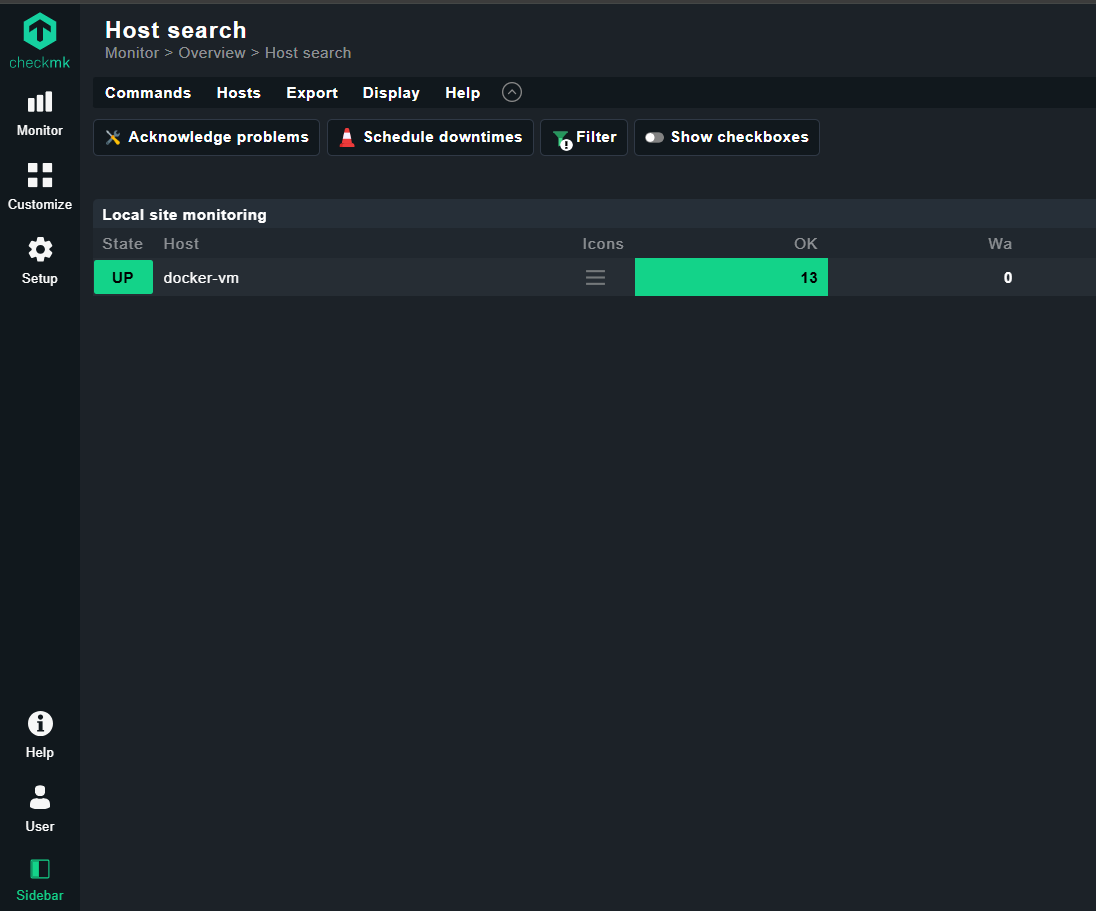
\includegraphics[width=0.85\textwidth]{scenario1_host_ok.png}
    \caption{De host blijft bereikbaar en wordt als OK weergegeven in Checkmk}
    \label{fig:scenario1_host_ok}
\end{figure}

\begin{figure}[H]
    \centering
    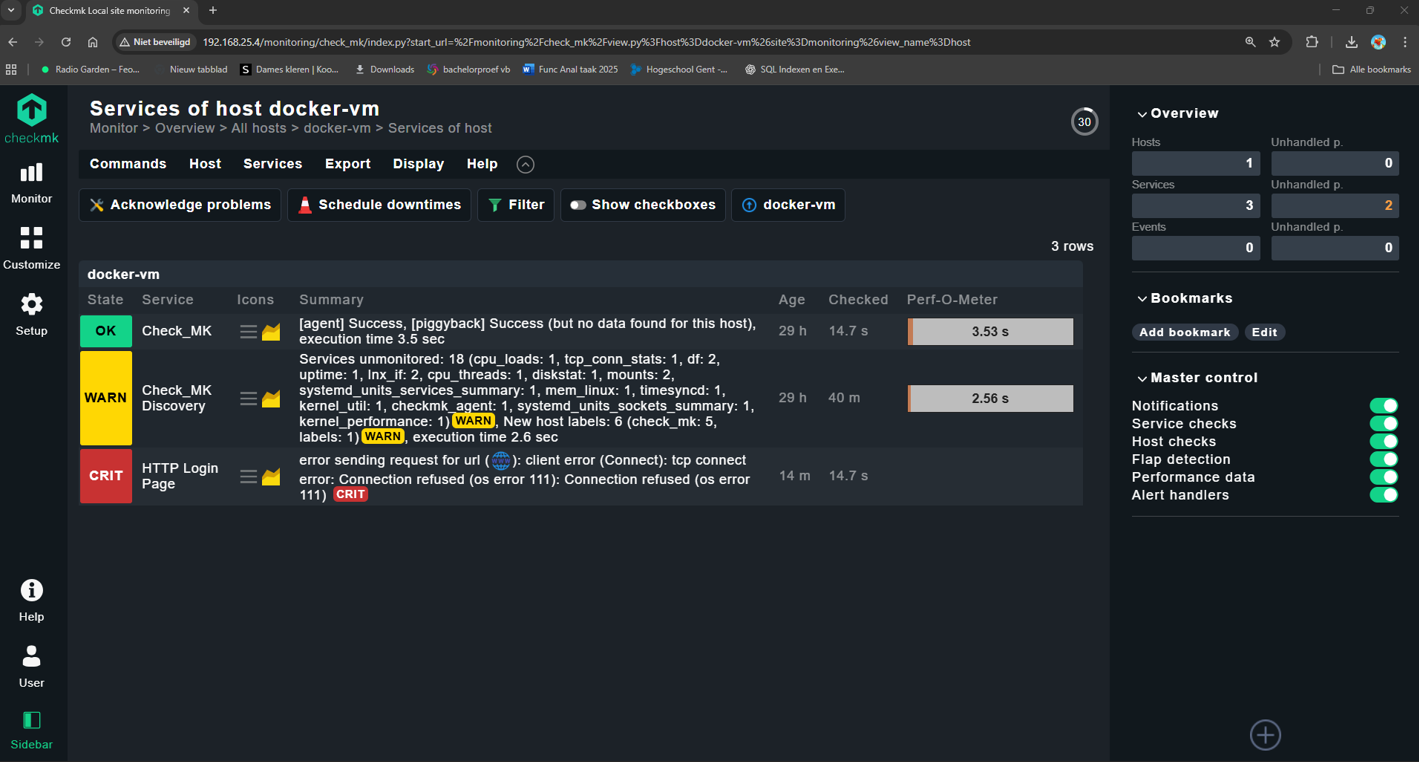
\includegraphics[width=0.85\textwidth]{scenario1_service_crit.png}
    \caption{De HTTP-service wordt als CRIT gemarkeerd wanneer de applicatie niet bereikbaar is}
    \label{fig:scenario1_service_crit}
\end{figure}

\begin{figure}[H]
    \centering
    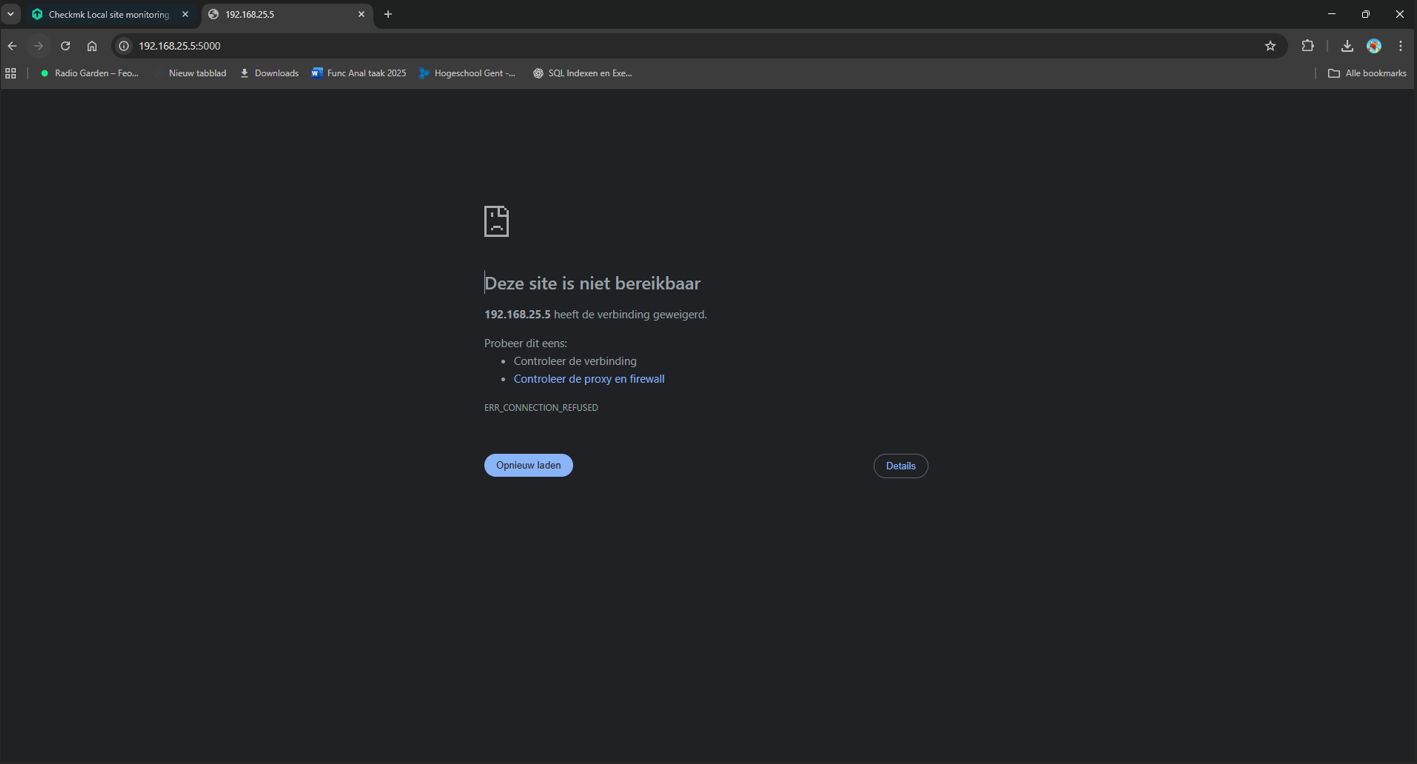
\includegraphics[width=0.75\textwidth]{scenario1_error.png}
    \caption{Foutmelding die aangeeft dat de webapplicatie niet bereikbaar is}
    \label{fig:scenario1_error}
\end{figure}

\subsubsection{Interpretatie}

Dit scenario toont aan dat traditionele monitoring in staat is om storingen op applicatieniveau te detecteren wanneer een service onbeschikbaar wordt.
Daarnaast wordt duidelijk dat er een onderscheid wordt gemaakt tussen de infrastructuur- en applicatieniveau. De host blijft als OK gemarkeerd staan, terwijl de webservice als CRIT wordt weergegeven.
Hieruit kan worden geconcludeerd dat traditionele monitoring weliswaar effectief is in het detecteren van beschikbaarheidsproblemen, maar onvoldoende inzicht biedt in de daadwerkelijke functionaliteit van de applicatie. Dit impliceert dat traditionele monitoring een onderscheid maakt tussen netwerkbereikbaarheid enerzijds en de feitelijke beschikbaarheid van de dienst anderzijds
Dit toont aan dat traditionele monitoring een onderscheid maakt tussen netwerkbereikbaarheid en servicebeschikbaarheid.




\subsection{Scenario 2: Databasefout (traditionele monitoring)}

\subsubsection{Beschrijving}

In dit scenario wordt een storing gesimuleerd op databaseniveau door de databasecontainer te stoppen, terwijl de webapplicatie actief blijft.

Het doel van dit scenario is om te onderzoeken in welke mate traditionele monitoring in staat is om fouten te detecteren die zich voordoen in de backend van een applicatie, zonder dat de webservice zelf onbeschikbaar wordt.

\subsubsection{Uitvoering}

De databasecontainer werd handmatig gestopt met behulp van Docker. Hierdoor kon de webapplicatie geen verbinding meer maken met de database.

De webserver bleef echter actief en bleef reageren op HTTP-verzoeken op poort 5000.

\subsubsection{Observatie}

De HTTP Login Check werd automatisch uitgevoerd door Checkmk en detecteerde onmiddellijk dat de webapplicatie geen correcte verbinding meer kon maken met de database.

Dit zorgde ervoor dat de status van de check automatisch naar \texttt{CRIT} veranderde, zonder dat de webpagina manueel geopend moest worden in een browser.

De fout werd rechtstreeks zichtbaar binnen de monitoringomgeving, waardoor het probleem automatisch gedetecteerd werd nog voordat een gebruiker effectief probeerde in te loggen.

Dit gedrag wordt geïllustreerd in Figuur~\ref{fig:scenario2_http_ok} en Figuur~\ref{fig:scenario2_db_error}.

\begin{figure}[H]
    \centering
    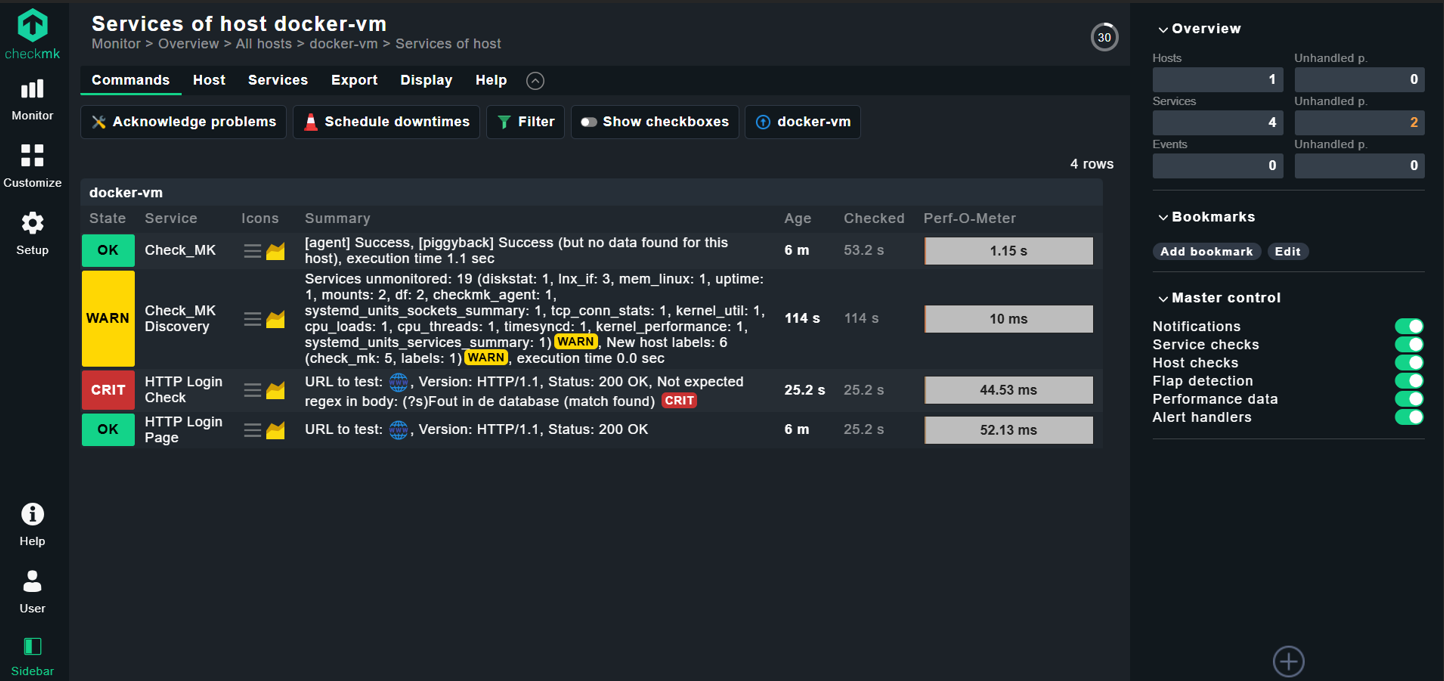
\includegraphics[width=0.85\textwidth]{scenario2_http_ok.png}
    \caption{De HTTP-service blijft als OK weergegeven, aangezien de webserver nog steeds bereikbaar is. Tegelijkertijd wordt de databasegerelateerde check als CRIT gemarkeerd.}
    \label{fig:scenario2_http_ok}
\end{figure}

\begin{figure}[H]
    \centering
    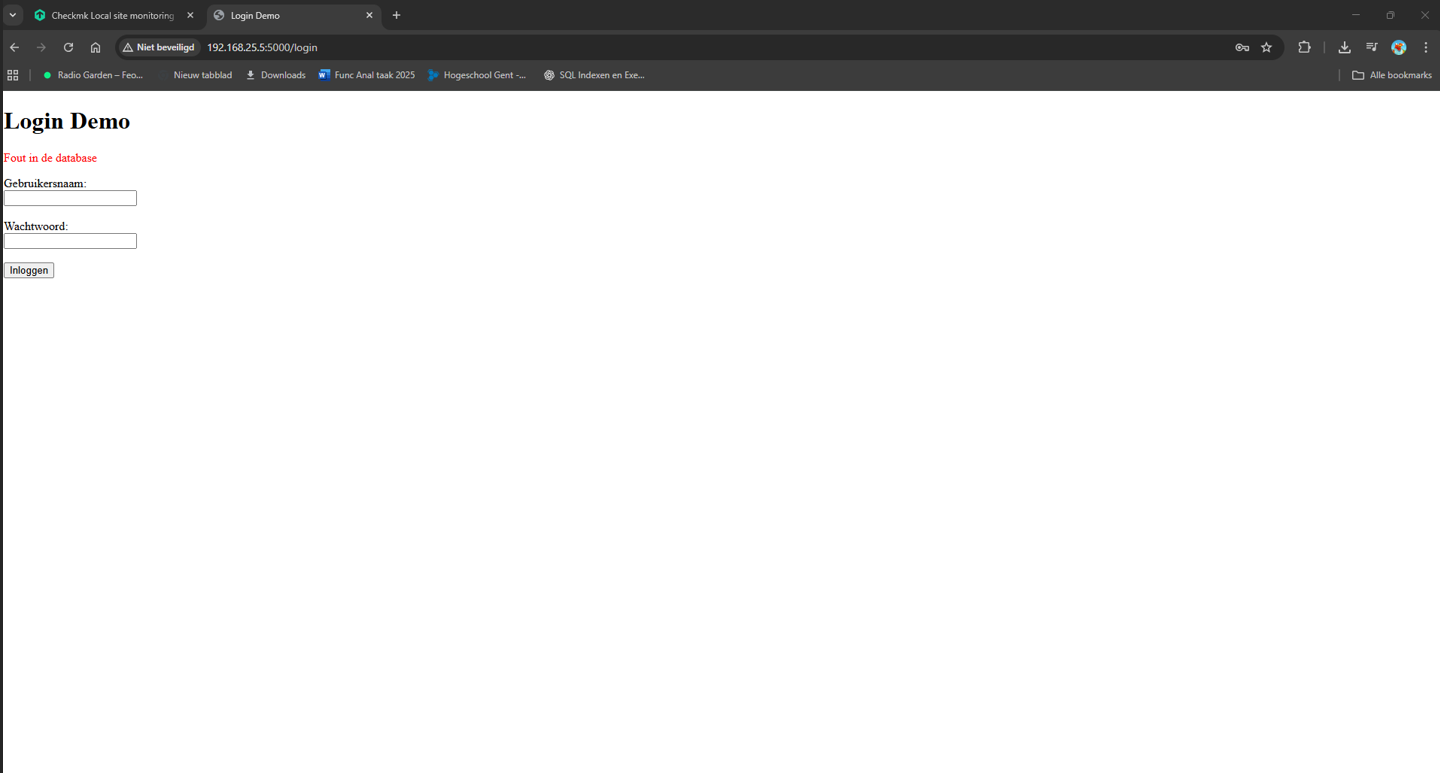
\includegraphics[width=0.85\textwidth]{scenario2_db_error.png}
    \caption{Foutmelding in de webapplicatie ten gevolge van een databaseprobleem}
    \label{fig:scenario2_db_error}
\end{figure}

\subsubsection{Interpretatie}

Dit scenario toont aan dat traditionele monitoring in staat is om een probleem te detecteren wanneer de verwachte inhoud van de webpagina afwijkt van de normale toestand.

Hoewel de webserver zelf nog bereikbaar is, wordt de HTTP-service als CRIT gemarkeerd omdat de inhoud van de pagina niet overeenkomt met de verwachte output. In dit geval wordt een foutmelding weergegeven als gevolg van een databaseprobleem.

Dit wijst erop dat traditionele monitoring uitgebreid kan worden met inhoudsgebaseerde controles, waardoor ook bepaalde applicatiefouten gedetecteerd kunnen worden.

Desondanks blijft deze aanpak beperkt, aangezien enkel vooraf gedefinieerde controles worden uitgevoerd en er geen volledig inzicht is in de gebruikersinteractie of de volledige functionaliteit van de applicatie.



\subsection{Scenario 3: Trage webapplicatie (traditionele monitoring)}

\subsubsection{Beschrijving}

In dit scenario wordt een performantieprobleem gesimuleerd door een kunstmatige vertraging toe te voegen aan de webapplicatie. De applicatie blijft hierdoor functioneel en bereikbaar, maar reageert trager voor de eindgebruiker.

Het doel van dit scenario is om te onderzoeken in welke mate traditionele monitoring in staat is om niet alleen beschikbaarheid maar ook performantieproblemen te detecteren.

\subsubsection{Uitvoering}

De webapplicatie werd vertraagd door in de backend een wachttijd toe te voegen. Hierdoor bleef de webserver beschikbaar op poort 5000, maar duurde het langer vooraleer de loginpagina volledig werd weergegeven.

De HTTP-check bleef de webservice controleren, maar hield daarnaast ook rekening met de responstijd van de webpagina.

\subsubsection{Observatie}

Wanneer de webapplicatie normaal functioneerde, bedroeg de responstijd van de loginpagina ongeveer 19,08 ms. Dit resulteerde in een OK-status binnen Checkmk.

Na het toevoegen van de kunstmatige vertraging steeg de responstijd tot ongeveer 5,02 s. Hierdoor werd de service als problematisch gemarkeerd, omdat de responstijd de ingestelde drempelwaarde overschreed.

Dit gedrag wordt geïllustreerd in Figuur~\ref{fig:scenario3_fast} en Figuur~\ref{fig:scenario3_slow}.

\begin{figure}[H]
    \centering
    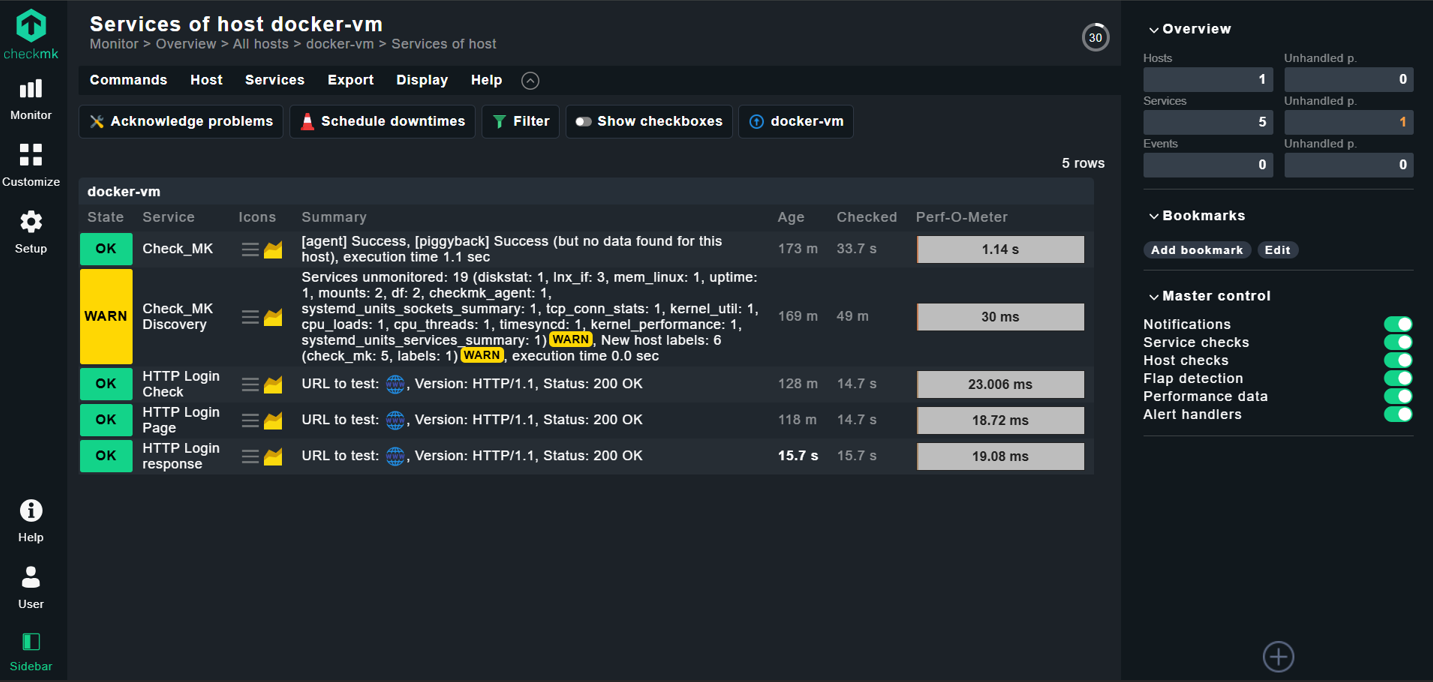
\includegraphics[width=0.85\textwidth]{scenario3_fast.png}
    \caption{De webapplicatie reageert normaal met een responstijd van ongeveer 19,08 ms}
    \label{fig:scenario3_fast}
\end{figure}

\begin{figure}[H]
    \centering
    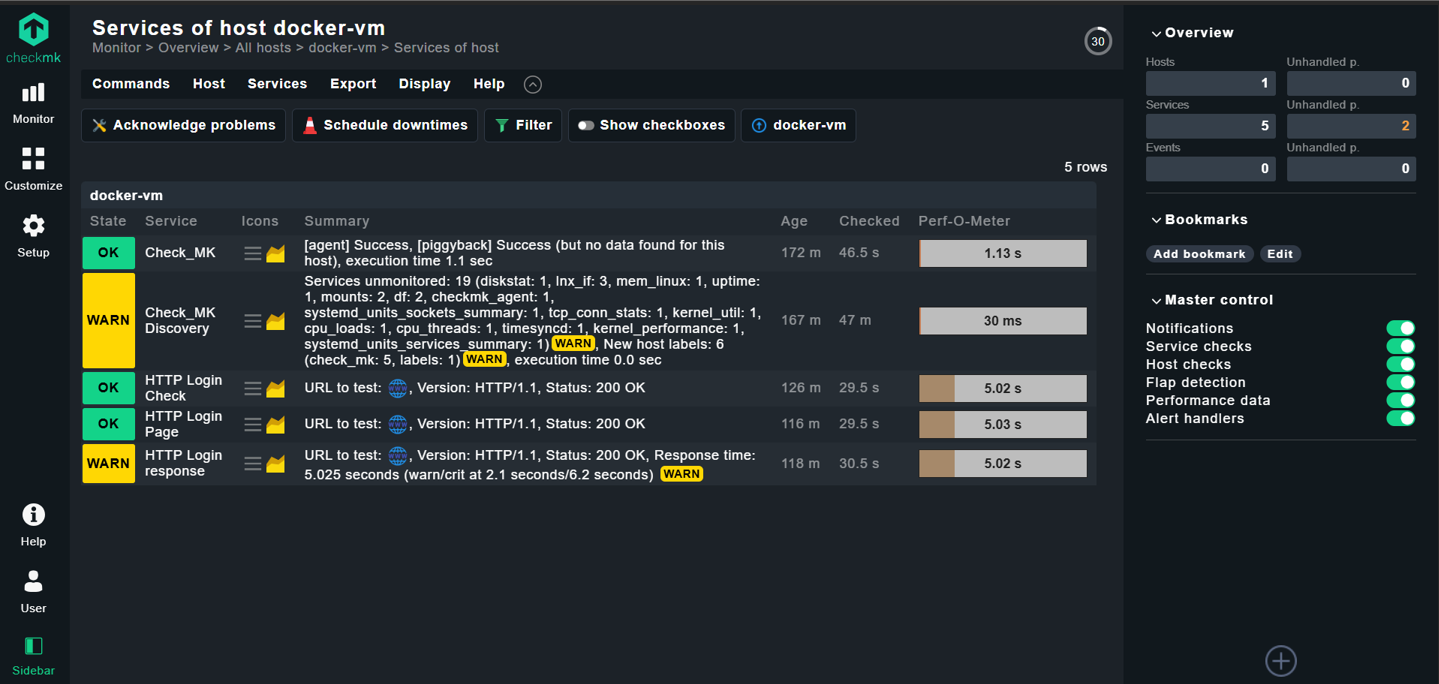
\includegraphics[width=0.85\textwidth]{scenario3_slow.png}
    \caption{De webapplicatie reageert traag met een responstijd van ongeveer 5,02 s}
    \label{fig:scenario3_slow}
\end{figure}

\subsubsection{Interpretatie}

Dit scenario toont aan dat traditionele monitoring niet enkel gebruikt kan worden om beschikbaarheidsproblemen te detecteren, maar ook om performantieproblemen zichtbaar te maken.

Hoewel de webapplicatie technisch gezien bereikbaar bleef, had de verhoogde responstijd een negatieve impact op de gebruikerservaring. Door drempelwaarden te configureren op de HTTP-responstijd kan Checkmk vertragingen detecteren en de service als WARN of CRIT markeren.

Hieruit kan geconcludeerd worden dat traditionele monitoring geschikt is om eenvoudige performantieproblemen op serviceniveau te detecteren. De beperking blijft echter dat deze meting voornamelijk de responstijd van de service weergeeft en geen volledige gebruikersinteractie simuleert.

\subsection{Scenario 4: Hoge CPU-belasting (traditionele monitoring)}

\subsubsection{Beschrijving}

In dit scenario wordt een infrastructuurprobleem gesimuleerd door de CPU-belasting van de virtuele machine kunstmatig te verhogen. 

Het doel van dit scenario is om te onderzoeken in welke mate traditionele monitoring in staat is om resource-gerelateerde problemen zoals bijvoorbeeld een hoge CPU-belasting, te detecteren.

\subsubsection{Uitvoering}

De CPU-belasting werd verhoogd door een stressprogramma uit te voeren op de virtuele machine. Hierdoor werd een behoorlijk groot deel van de beschikbare CPU-capaciteit gebruikt gedurende een bepaalde periode.

De webapplicatie bleef tijdens deze test actief en bereikbaar, maar reageerde trager.

\subsubsection{Observatie}

De centrale monitoringserver ontving via de Checkmk-agent informatie over de verhoogde CPU load en CPU utilization.

De CPU load steeg tot boven de normale waarden, terwijl ook het CPU-gebruik percentage aanzienlijk verhoogde. Wanneer de ingestelde drempelwaarden werden overschreden, werd de service als WARN of CRIT gemarkeerd.

Dit gedrag wordt geïllustreerd in Figuur~\ref{fig:scenario4_cpu_ok} en Figuur~\ref{fig:scenario4_cpu_high}.

\begin{figure}[H]
    \centering
    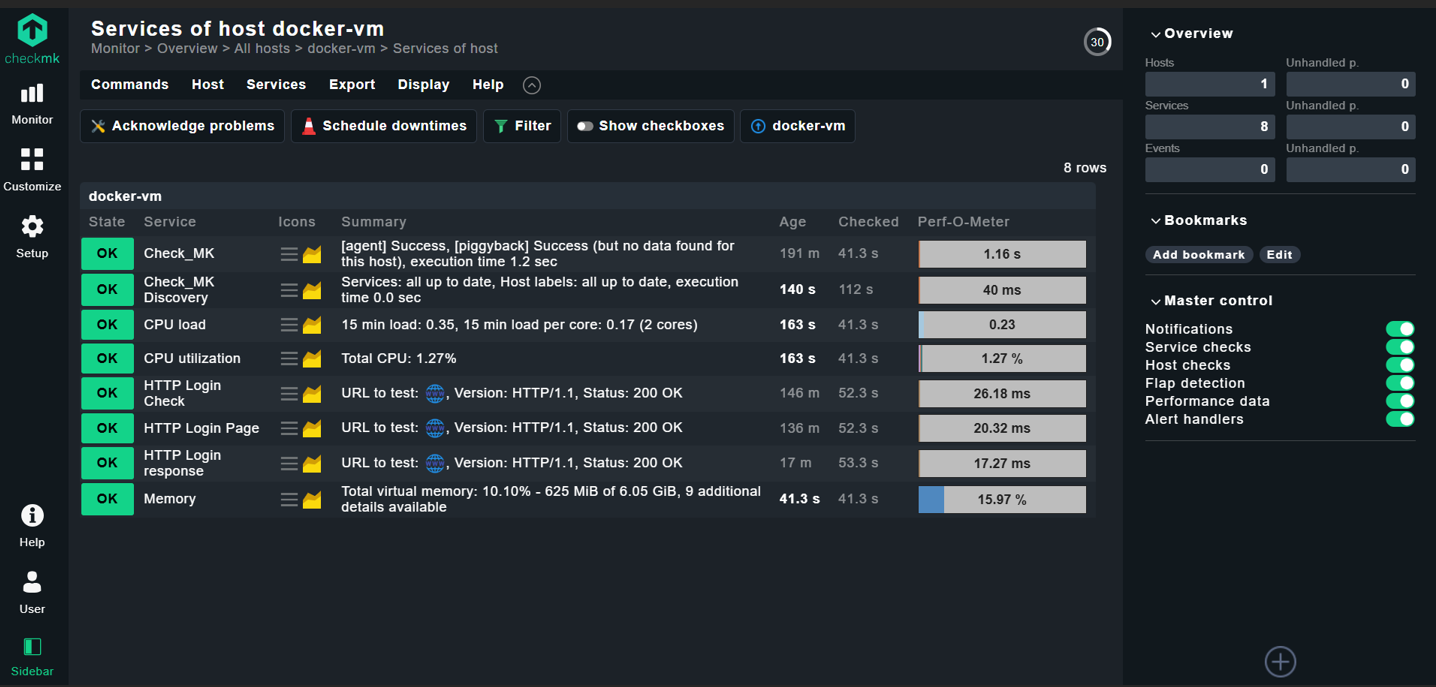
\includegraphics[width=0.85\textwidth]{scenario4_cpu_ok.png}
    \caption{Normale CPU-belasting met lage load en utilization}
    \label{fig:scenario4_cpu_ok}
\end{figure}

\begin{figure}[H]
    \centering
    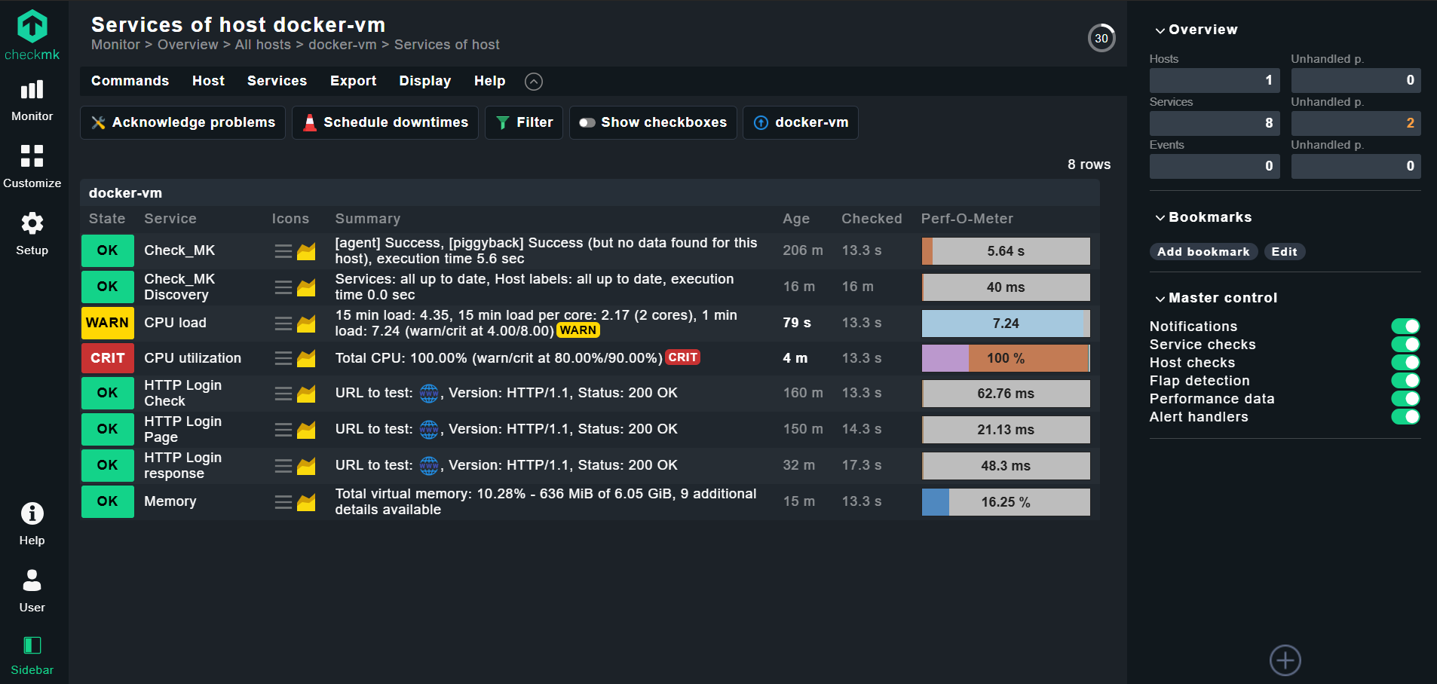
\includegraphics[width=0.85\textwidth]{scenario4_cpu_high.png}
    \caption{Hoge CPU-belasting waarbij de ingestelde drempelwaarden overschreden worden}
    \label{fig:scenario4_cpu_high}
\end{figure}

\subsubsection{Interpretatie}

Dit scenario toont aan dat traditionele monitoring zeer geschikt is voor het detecteren van infrastructuurproblemen zoals een hoge CPU-belasting.

In tegenstelling tot applicatieproblemen, die afhankelijk zijn van configuratie of inhoudscontroles, kunnen resourceproblemen direct gemeten worden aan de hand van systeemparameters.

Hierdoor kan traditionele monitoring snel en betrouwbaar waarschuwingen genereren wanneer de belasting van het systeem te hoog wordt.

De beperking blijft echter dat er geen directe koppeling wordt gemaakt tussen de verhoogde CPU-belasting en de impact op de applicatie of de gebruikerservaring.

\subsection{Scenario 5: Verlies van connectiviteit tussen applicatie en database (traditionele monitoring)}

\subsubsection{Beschrijving}

In dit scenario wordt een connectiviteitsprobleem tussen de webapplicatie en de database gesimuleerd.

Het doel van dit scenario is om te onderzoeken in welke mate traditionele monitoring in staat is om problemen tussen verschillende componenten van de applicatie correct te detecteren.

\subsubsection{Uitvoering}

De connectiviteit tussen de webapplicatie en de database werd verstoord door een foutieve configuratie van de databasehost in de applicatieomgeving.

Hierdoor bleef de databasecontainer technisch actief, maar kon de webapplicatie geen verbinding meer maken met de database.

Tijdens dit scenario werden verschillende traditionele monitoringchecks uitgevoerd, waaronder een TCP-check op poort 3306, de standaard netwerkpoort die gebruikt wordt door de MySQL-database. Daarnaast werd ook een HTTP-inhoudscontrole uitgevoerd op de webapplicatie.

\subsubsection{Observatie}

De TCP-check op poort 3306 gaf nog steeds de status \textit{OK}, wat aantoont dat de database technisch actief bleef en verbindingen accepteerde.

De HTTP-inhoudscontrole detecteerde echter dat de applicatie een foutmelding weergaf als gevolg van het connectiviteitsprobleem tussen applicatie en database.

De service werd als \textit{CRIT} gemarkeerd.

Dit gedrag wordt geïllustreerd in Figuur~\ref{fig:trad_scenario5_tcp_ok}.

\begin{figure}[H]
    \centering
    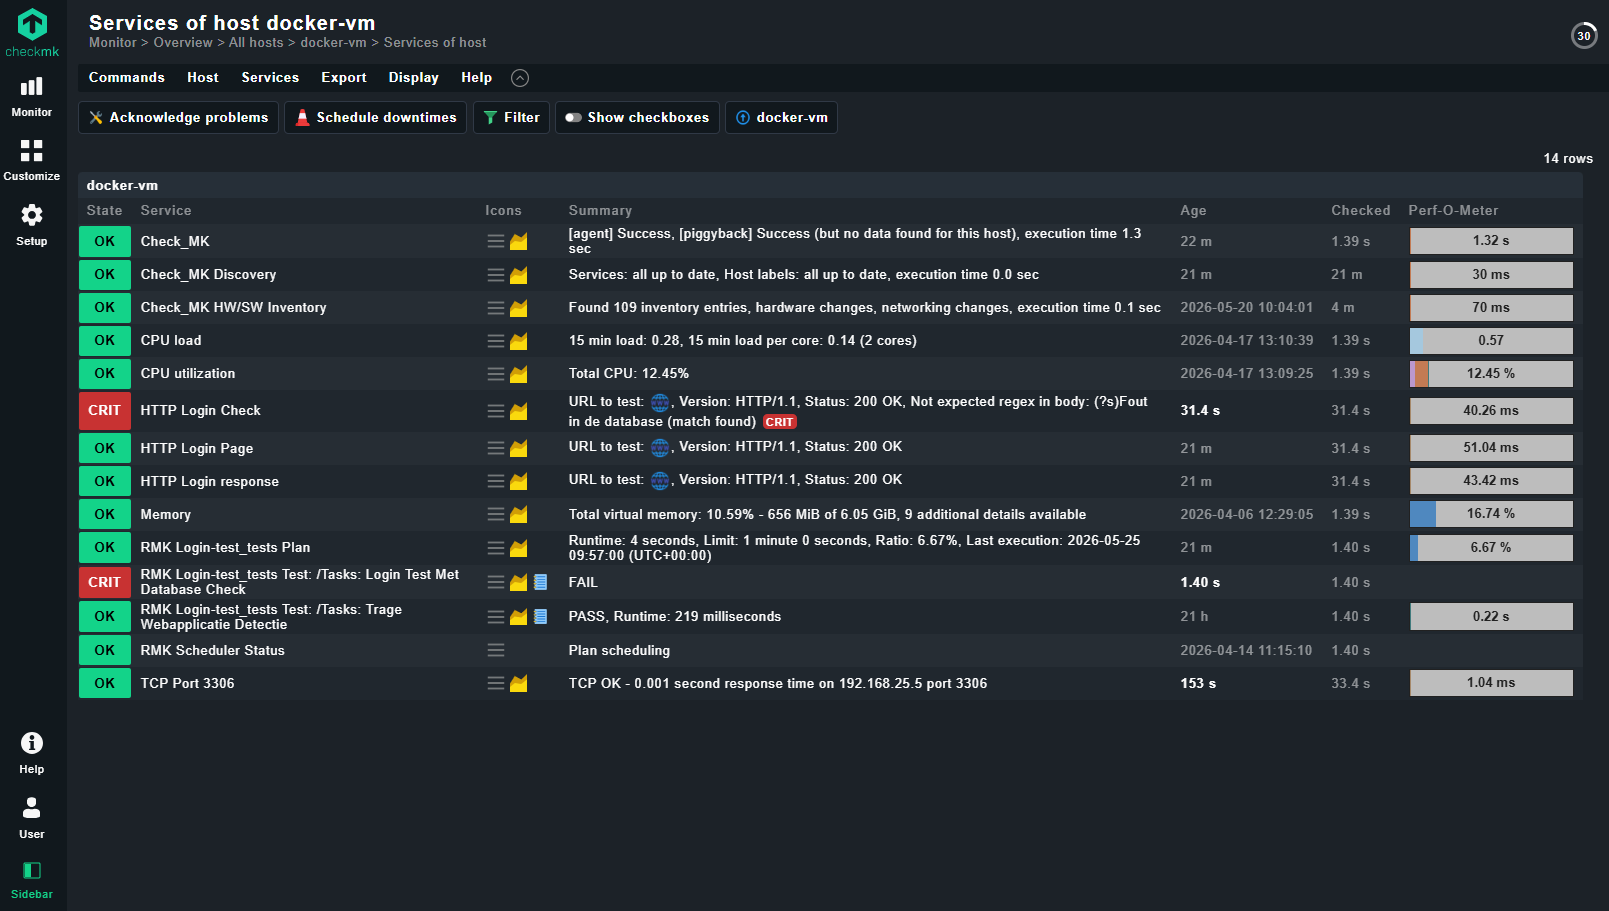
\includegraphics[width=0.9\textwidth]{scenario5_tcp_ok.png}
    \caption{De database blijft technisch bereikbaar via de TCP-check op poort 3306 maar er kan niet ingelogd worden.}
    \label{fig:trad_scenario5_tcp_ok}
\end{figure}

\subsubsection{Interpretatie}

Dit scenario toont aan dat traditionele monitoring verschillende gespecialiseerde controles vereist om zowel de beschikbaarheid van de database als de connectiviteit tussen applicatie en database correct te evalueren.

Hoewel de database technisch actief bleef, kon de applicatie geen verbinding meer maken met de database.

Door afzonderlijke TCP- en HTTP-controles te combineren kon het probleem correct geanalyseerd worden binnen de monitoringomgeving.

\subsection{Scenario 6: Redirectloop na login (traditionele monitoring)}

\subsubsection{Beschrijving}

In dit scenario wordt een functioneel probleem binnen de webapplicatie gesimuleerd waarbij gebruikers na een succesvolle login opnieuw teruggestuurd worden naar de loginpagina in plaats van naar de verwachte succespagina.

Het doel van dit scenario is om te onderzoeken in welke mate traditionele monitoring functionele problemen binnen een gebruikersflow kan detecteren.

\subsubsection{Uitvoering}

De applicatielogica werd aangepast zodat gebruikers na een correcte login niet doorgestuurd werden naar de succespagina, maar terug op de loginpagina terechtkwamen.

Hierdoor bleef de webapplicatie technisch volledig bereikbaar en retourneerde de webserver correcte HTTP-responses.

Tijdens dit scenario werden traditionele monitoringchecks uitgevoerd, waaronder HTTP-checks en TCP-connectiviteitschecks voor de database.

\subsubsection{Observatie}

De traditionele monitoringchecks bleven de status \textit{OK} weergeven. Zowel de webserver als de database bleven technisch bereikbaar en de webpagina retourneerde correcte HTTP-responses zonder foutmeldingen.

Hoewel de loginflow functioneel niet correct werkte voor de eindgebruiker, detecteerde traditionele monitoring geen probleem.

Dit gedrag wordt geïllustreerd in Figuur~\ref{fig:trad_scenario6_OK_trad}.

\begin{figure}[H]
    \centering
    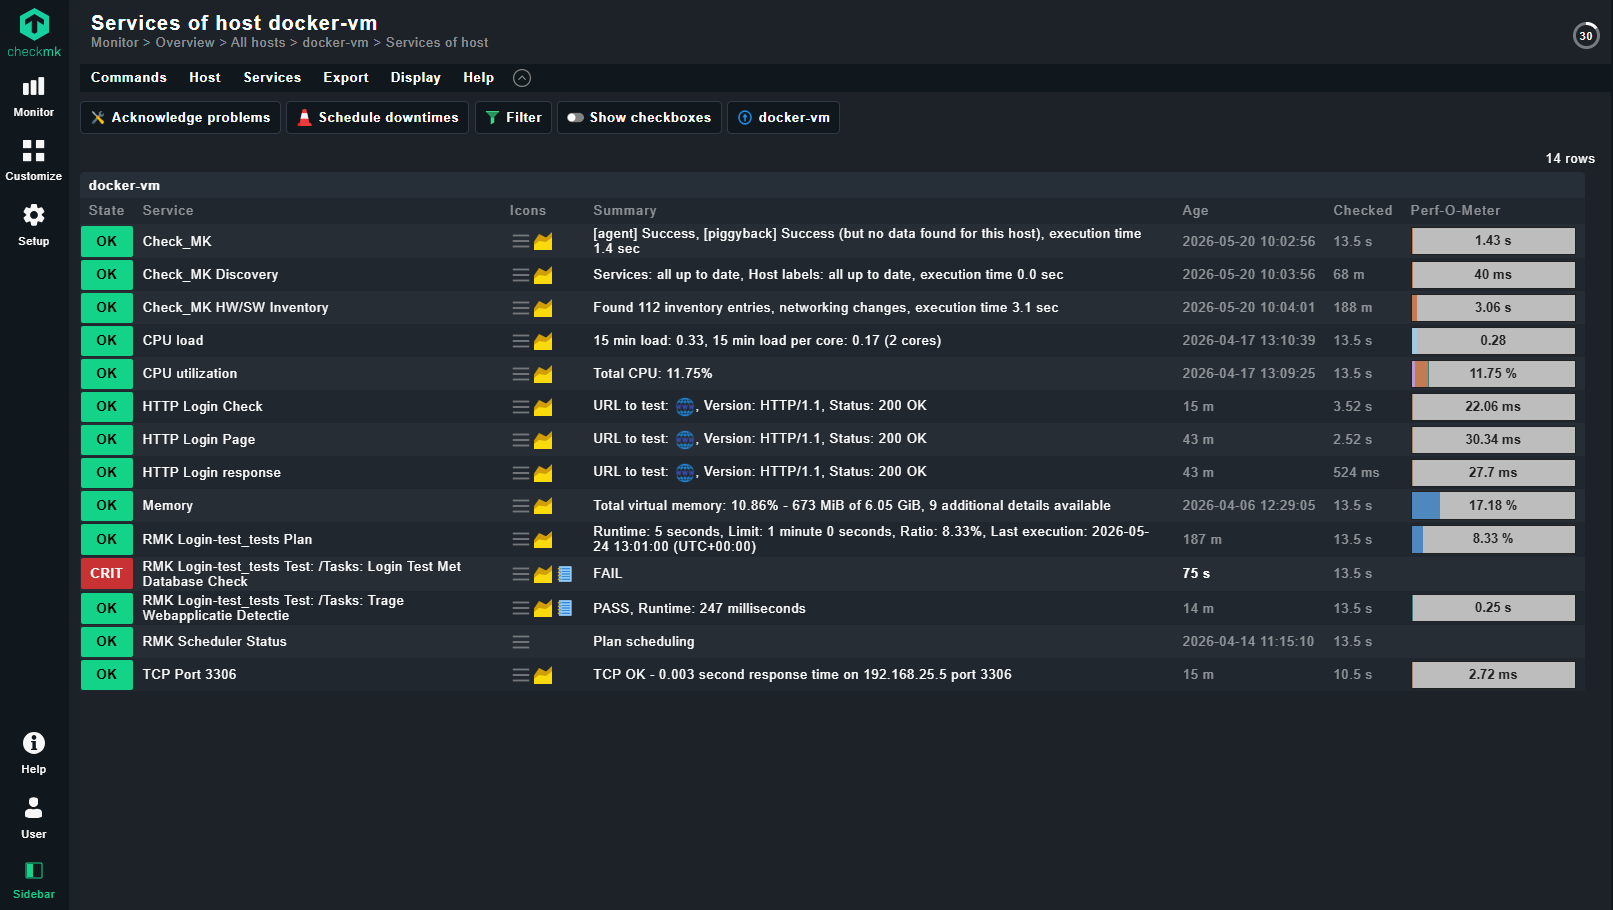
\includegraphics[width=0.95\textwidth]{Scenario6_checkmkerror.png}
    \caption{Traditionele monitoring detecteert geen probleem omdat de services technisch bereikbaar blijven.}
    \label{fig:trad_scenario6_OK_trad}
\end{figure}

\subsubsection{Interpretatie}

Dit scenario toont aan dat traditionele monitoring voornamelijk controleert of services technisch bereikbaar blijven en correcte HTTP-responses retourneren.

Functionele problemen binnen de gebruikersflow worden hierbij niet automatisch gedetecteerd zolang de infrastructuur en webservices operationeel blijven.

Dit toont aan dat technische beschikbaarheid niet noodzakelijk betekent dat een applicatie ook functioneel correct werkt voor de eindgebruiker.

\section{End-to-end monitoring met Robotmk}

Na het analyseren van de verschillende scenario’s met traditionele monitoring, worden in dit deel dezelfde scenario’s opnieuw uitgevoerd met behulp van end-to-end monitoring via Robotmk.

Het doel hiervan is om een directe vergelijking te maken tussen beide monitoringsmanieren. Door identieke situaties te simuleren, kan onderzocht worden in welke mate end-to-end monitoring verschilt van traditionele monitoring op vlak van detectie/detectiesnelheid, nauwkeurigheid en relevantie voor de eindgebruiker.

In tegenstelling tot traditionele monitoring, waarbij afzonderlijke componenten zoals services en systeemresources worden gecontroleerd, gedraagt end-to-end monitoring zich meer als een echte gebruiker die met de applicatie werkt. Hierbij wordt niet enkel gekeken naar de beschikbaarheid van de applicatie, maar ook naar de correcte werking ervan vanuit het perspectief van de eindgebruiker.

Binnen deze proof-of-concept worden de uitgevoerde gebruikersflows beschouwd als een vorm van end-to-end tracing. Hierbij wordt stap voor stap opgevolgd hoe een gebruiker met de applicatie interacteert en waar binnen deze flow eventuele fouten of vertragingen optreden.

De zes eerder uitgewerkte scenario’s worden daarom opnieuw getest met Robotmk:
\begin{itemize}
    \item Uitval van de webapplicatie
    \item Databasefout
    \item Trage webapplicatie
    \item Hoge CPU-belasting
    \item Verlies van connectiviteit tussen applicatie en database
    \item Redirectloop na login
\end{itemize}

Op basis van deze tests wordt geanalyseerd hoe end-to-end monitoring zich verhoudt tot traditionele monitoring en in welke situaties deze aanpak een meerwaarde biedt.

\subsubsection{Overzicht van Robotmk componenten}

Figuur~\ref{fig:robotmk_services} toont een overzicht van de Robotmk-gerelateerde services binnen Checkmk. Twee belangrijke componenten hierin zijn de \texttt{RMK Login-test\_tests Plan} en de \texttt{RMK Scheduler Status}.

\begin{figure}[H]
    \centering
    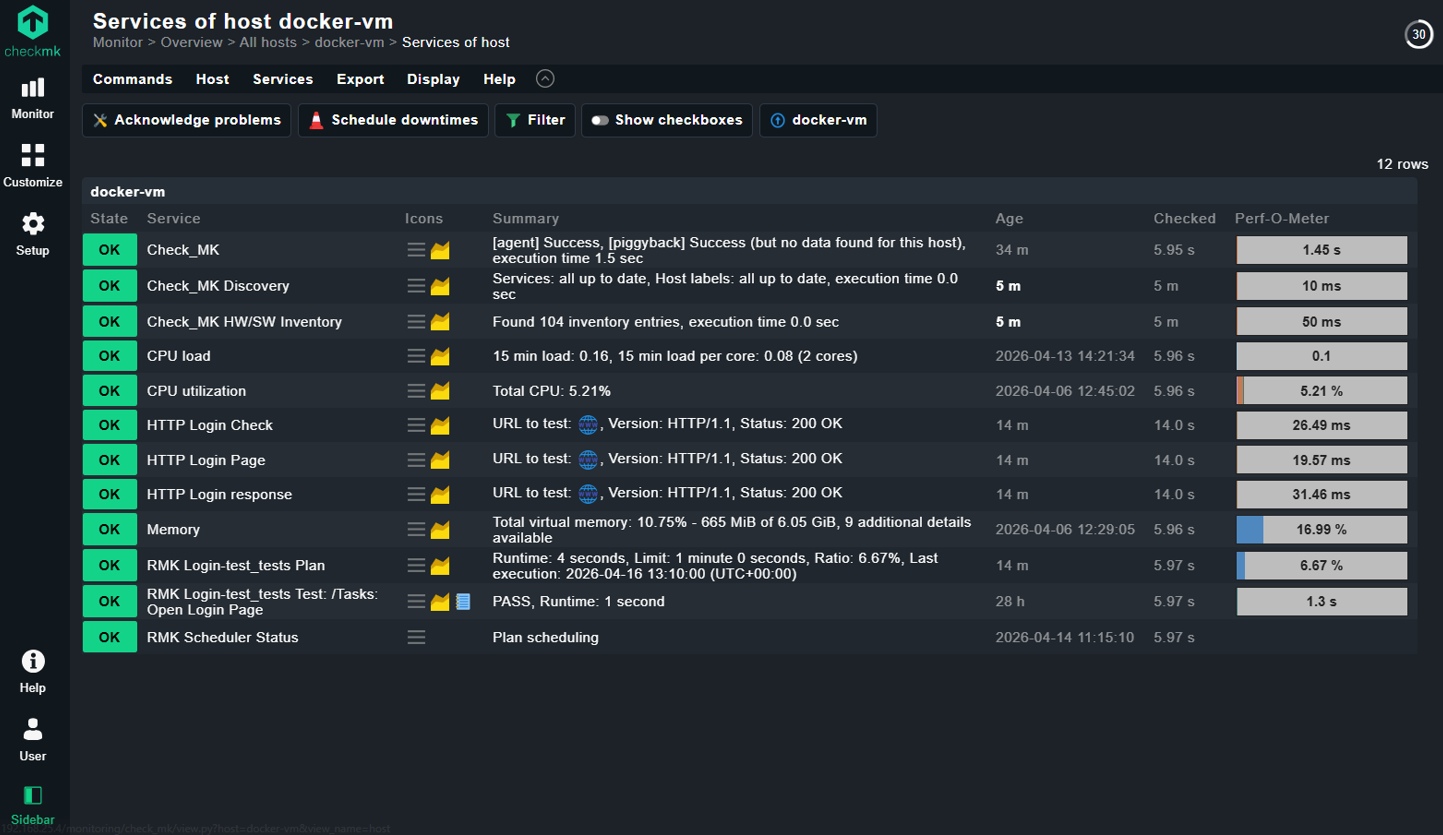
\includegraphics[width=0.95\textwidth]{robotmk_services.png}
    \caption{Overzicht van Robotmk services binnen Checkmk}
    \label{fig:robotmk_services}
\end{figure}

De service \texttt{RMK Login-test\_tests Plan} beheert de planning van de end-to-end tests. Deze component bepaalt wanneer een test uitgevoerd moet worden, wanneer de volgende uitvoering gepland staat en controleert of de test correct en tijdig gestart is.

De \texttt{RMK Scheduler Status} vormt het centrale onderdeel van Robotmk. Deze service is verantwoordelijk voor het effectief uitvoeren van de tests, het voorkomen van overlappende testuitvoeringen en het verwerken van de resultaten. Daarnaast houdt deze component de algemene status van de testuitvoering bij.

Samen zorgen deze twee componenten ervoor dat de end-to-end monitoring gestructureerd, betrouwbaar en periodiek wordt uitgevoerd.

\subsection{Scenario 1: Uitval van de webapplicatie (end-to-end monitoring)}

\subsubsection{Beschrijving}

In dit scenario wordt gecontroleerd of de webapplicatie correct functioneert vanuit het perspectief van de eindgebruiker. Hierbij wordt niet enkel nagegaan of de webpagina bereikbaar is, maar ook of de verwachte inhoud correct wordt weergegeven.

Het doel van dit scenario is om te onderzoeken hoe end-to-end monitoring een storing van de webapplicatie detecteert vanuit het perspectief van de eindgebruiker.

\subsubsection{Uitvoering}

De Robotmk-test werd uitgevoerd met behulp van een headless Chromium-browser. De test opent de loginpagina en controleert vervolgens of het label \texttt{Gebruikersnaam:} aanwezig is op de pagina.

Deze controle simuleert een eenvoudige gebruikersactie: een gebruiker opent de applicatie en verwacht het loginformulier correct te zien.

\subsubsection{Observatie}

De Robotmk-test geeft stap voor stap weer welke acties worden uitgevoerd. In de log is zichtbaar dat de browser correct wordt gestart, dat de webpagina wordt geopend en dat de tekst van het loginlabel wordt opgehaald.

De test faalt tijdens het controleren van de loginpagina. Robotmk kan de verwachte elementen van de webapplicatie niet correct detecteren, waardoor de gebruikersflow niet verder uitgevoerd kan worden. De test kreeg de status \textit{FAIL}.

Dit gedrag wordt weergegeven in Figuur~\ref{fig:e2e_scenario1_fail}.

\begin{figure}[H]
    \centering
    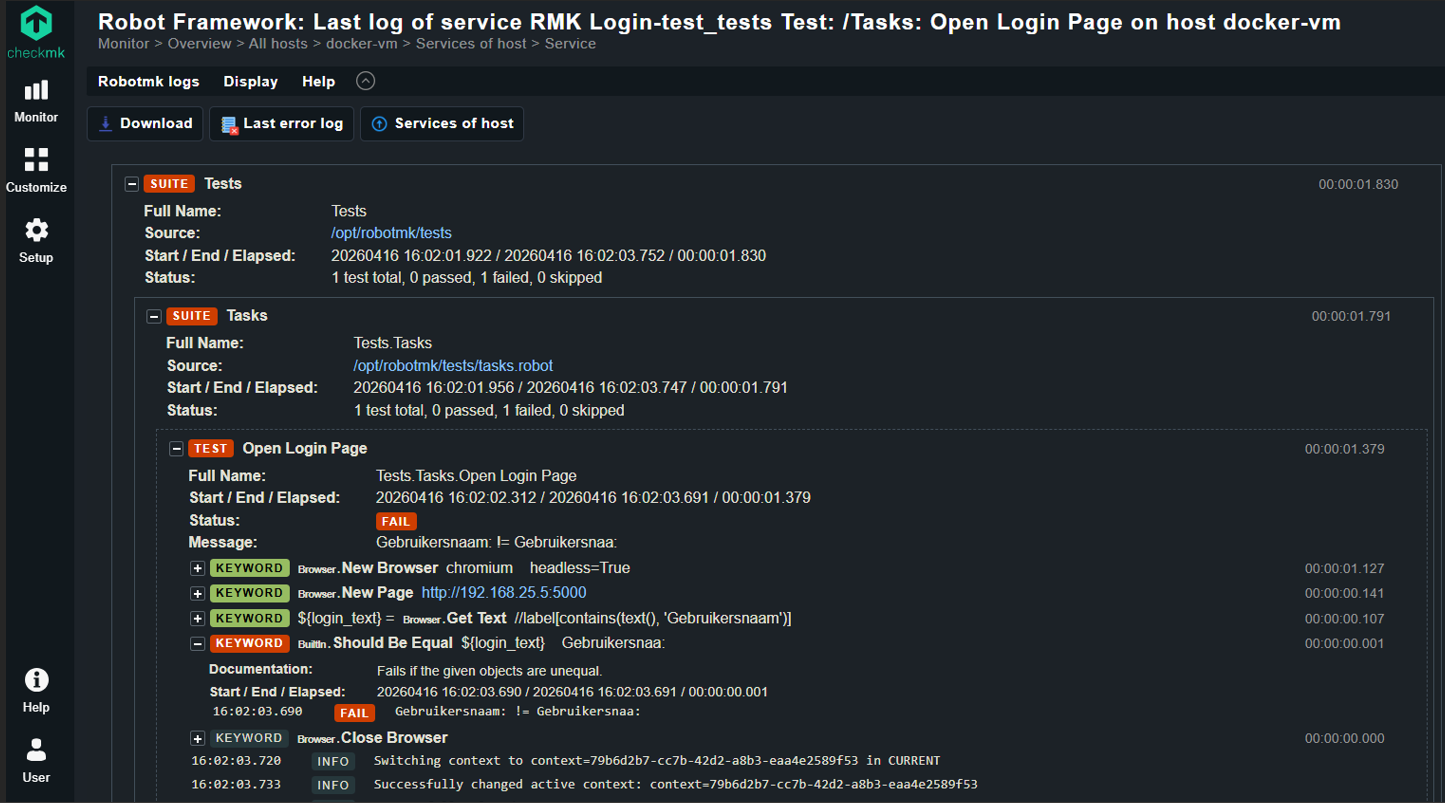
\includegraphics[width=0.85\textwidth]{e2e_scenario1_fail.png}
    \caption{Robotmk toont stap voor stap waar de end-to-end test faalt}
    \label{fig:e2e_scenario1_fail}
\end{figure}

\subsubsection{Interpretatie}

Dit scenario toont aan dat end-to-end monitoring meer inzicht biedt dan een eenvoudige beschikbaarheidscontrole. De webpagina kan technisch bereikbaar zijn, maar toch foutief functioneren wanneer de verwachte inhoud niet correct wordt weergegeven.

Een belangrijk voordeel van Robotmk is dat de uitvoering stap voor stap zichtbaar is in de testlog. Hierdoor kan niet alleen vastgesteld worden dat de test faalt, maar ook op welk punt in de gebruikersflow het probleem optreedt.

In dit geval wordt duidelijk dat de fout niet optreedt bij het openen van de pagina, maar bij het valideren van de verwachte tekst op de loginpagina. Dit maakt de foutanalyse concreter en gerichter dan bij een eenvoudige HTTP-check.

\subsection{Scenario 2: Databasefout (end-to-end monitoring)}

\subsubsection{Beschrijving}

In dit scenario wordt een storing gesimuleerd op databaseniveau, terwijl de webapplicatie zelf bereikbaar blijft.

Het doel van dit scenario is om te onderzoeken hoe end-to-end monitoring omgaat met fouten die zich voordoen binnen de applicatielogica, en hoe deze zichtbaar worden voor de gebruiker.

\subsubsection{Uitvoering}

De databasecontainer werd handmatig gestopt, waardoor de webapplicatie geen verbinding meer kon maken met de database.

Vervolgens werd de Robotmk-test uitgevoerd. Deze test opent de loginpagina, controleert of de pagina correct wordt weergegeven en voert een loginpoging uit met geldige gebruikersgegevens.

\subsubsection{Observatie}

De Robotmk-test toont stap voor stap de uitvoering van de gebruikersflow. In de log is zichtbaar dat de browser correct wordt gestart en dat de loginpagina succesvol wordt geopend.

De test faalt echter tijdens de verdere interactie met de applicatie. Na het inloggen, wordt er een foutmelding weergegeven op de pagina als gevolg van een probleem met de database.

Deze fout wordt gedetecteerd tijdens de validatiestap, waarbij gecontroleerd wordt of de pagina geen foutmelding bevat. Omdat de tekst \texttt{Fout in de database} aanwezig is, faalt de test.

De testlog geeft duidelijk weer welke stappen er zijn en welke stap slaagt of niet slaagt.
Dit gedrag wordt geïllustreerd in Figuur~\ref{fig:e2e_scenario2_ok}, Figuur~\ref{fig:e2e_scenario2_fail_2.0} en Figuur~\ref{fig:e2e_scenario2_fail}.

\begin{figure}[H]
    \centering
    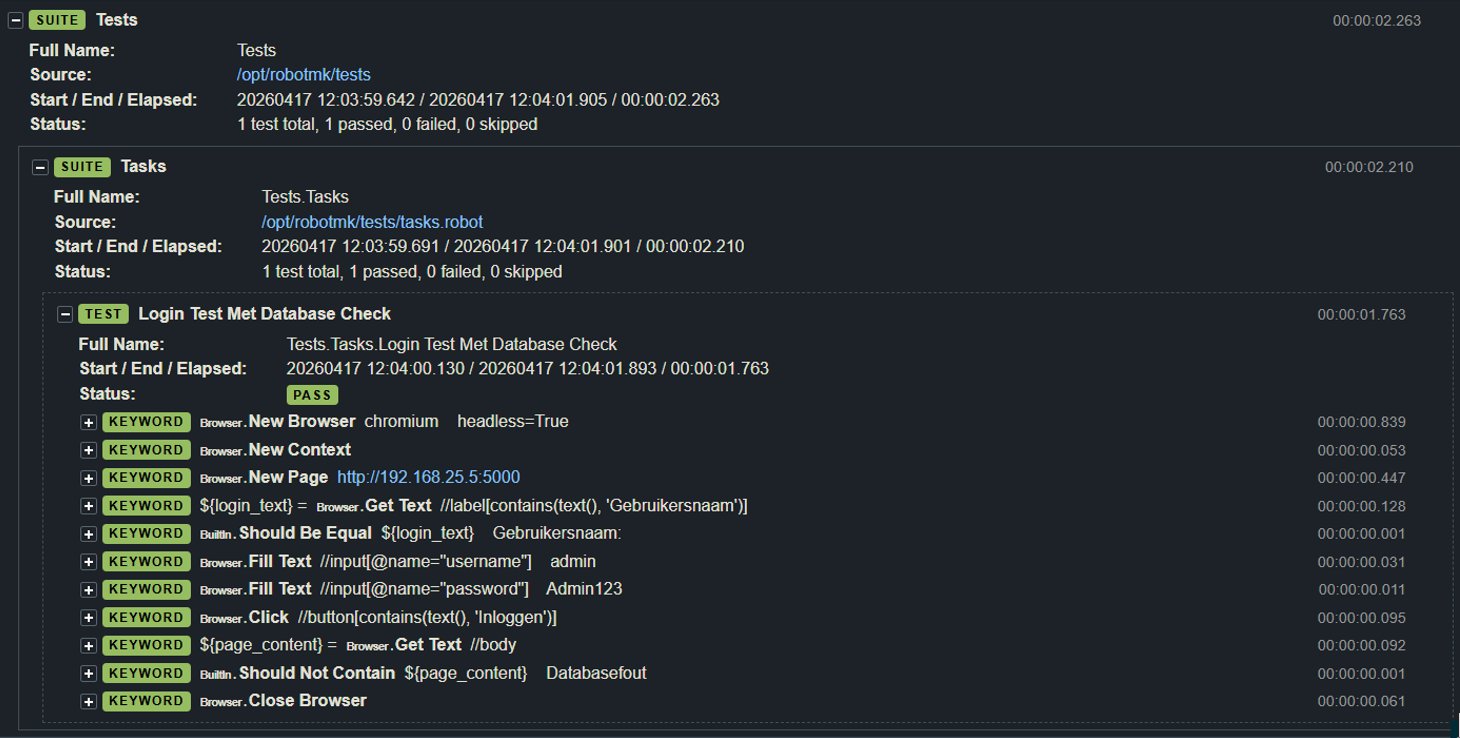
\includegraphics[width=0.85\textwidth]{e2e_scenario2_ok.png}
    \caption{Normaal verloop van de Robotmk test zonder de databasefout}
    \label{fig:e2e_scenario2_ok}
\end{figure}

\begin{figure}[H]
    \centering
    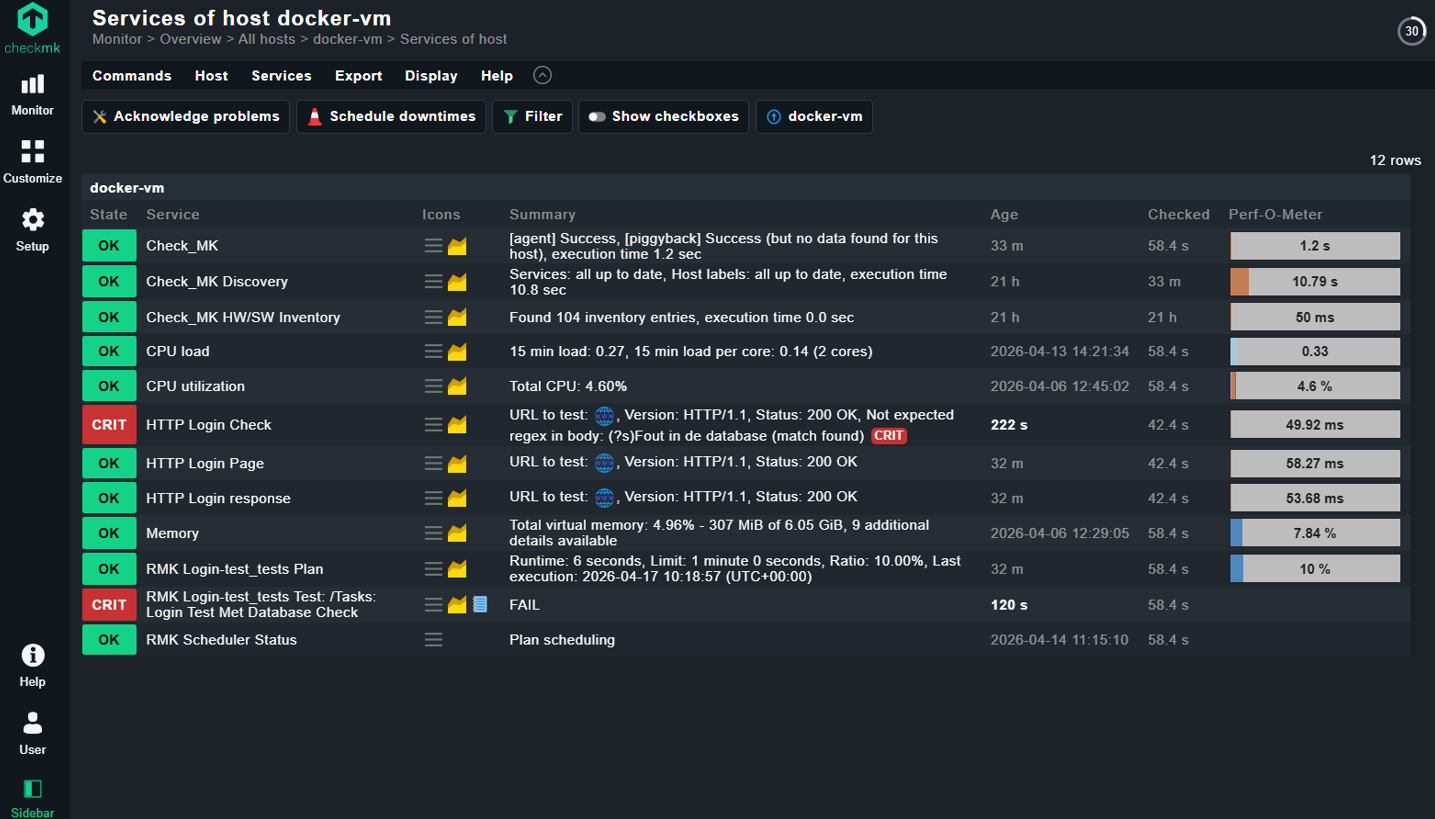
\includegraphics[width=0.85\textwidth]{e2e_scenario2_fail_2.0.png}
    \caption{Robotmk detecteert een databasefout en geeft dit weer}
    \label{fig:e2e_scenario2_fail_2.0}
\end{figure}

\begin{figure}[H]
    \centering
    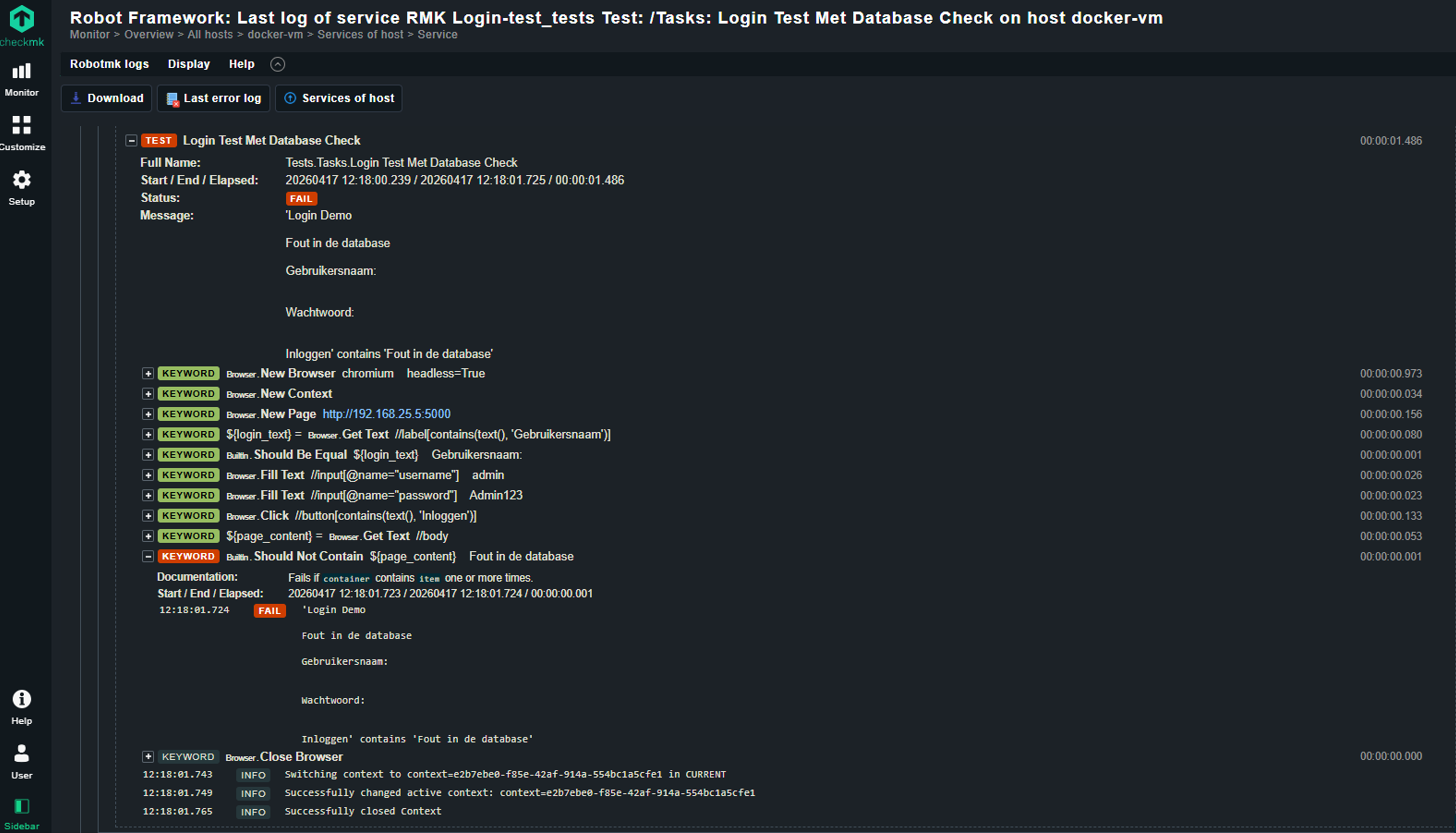
\includegraphics[width=0.85\textwidth]{e2e_scenario2_fail.png}
    \caption{Robotmk detecteert een databasefout tijdens de loginflow en toont de fout in de testlog}
    \label{fig:e2e_scenario2_fail}
\end{figure}


\subsubsection{Interpretatie}

Dit scenario toont aan dat end-to-end monitoring in staat is om fouten te detecteren die zich voordoen binnen de applicatie, zelfs wanneer de webservice zelf bereikbaar blijft.

In tegenstelling tot traditionele monitoring, waarbij dergelijke fouten afhankelijk zijn van vooraf geconfigureerde controles, wordt hier de volledige gebruikersflow geëvalueerd.

Een belangrijk voordeel is dat de testlog gedetailleerd weergeeft waar de fout optreedt. Hierdoor wordt niet alleen vastgesteld dat er een probleem is, maar ook in welke stap dit probleem zich bevindt.

Dit maakt het mogelijk om sneller en gerichter fouten te vinden en analyseren vanuit het perspectief van de eindgebruiker.

\subsection{Scenario 3: Trage webapplicatie (end-to-end monitoring)}

\subsubsection{Beschrijving}

In dit scenario wordt een performantieprobleem gesimuleerd door vertraging toe te voegen aan het laden van de webapplicatie.

Het doel van dit scenario is om te onderzoeken hoe end-to-end monitoring de gebruikerservaring evalueert wanneer de applicatie traag reageert.

\subsubsection{Uitvoering}

De webapplicatie werd vertraagd door een wachttijd toe te voegen in de backend. Hierdoor bleef de applicatie bereikbaar, maar duurde het langer vooraleer de loginpagina volledig geladen werd.

De Robotmk-test werd uitgevoerd en de tijd die nodig is om de pagina te openen en de verwachte elementen zichtbaar te maken werd bijgehouden.

\subsubsection{Observatie}

De Robotmk-test toont opnieuw stap voor stap de uitvoering van de gebruikersflow. In de log is zichtbaar dat de browser wordt gestart en dat de webpagina wordt geopend.

Door de toegevoegde vertraging duurt het echter langer vooraleer de verwachte elementen op de pagina zichtbaar zijn. Dit wordt gemeten tijdens de uitvoering van de test.

De totale uitvoeringstijd van de test stijgt merkbaar en kan de ingestelde drempelwaarde overschrijden. Wanneer dit gebeurt, wordt de test als CRIT beschouwd.

De testlog geeft duidelijk weer hoeveel tijd elke stap in beslag neemt, waardoor zichtbaar wordt waar de vertraging zich voordoet.

Hierbij blijft de applicatie technisch gezien bereikbaar, maar wordt de test als mislukt beschouwd vanwege de slechte performantie.

Dit gedrag wordt geïllustreerd in Figuur~\ref{fig:e2e_scenario3_OK}, Figuur~\ref{fig:e2e_scenario3_CRIT}, Figuur~\ref{fig:e2e_scenario3_fast} en Figuur~\ref{fig:e2e_scenario3_slow}.

\begin{figure}[H]
    \centering
    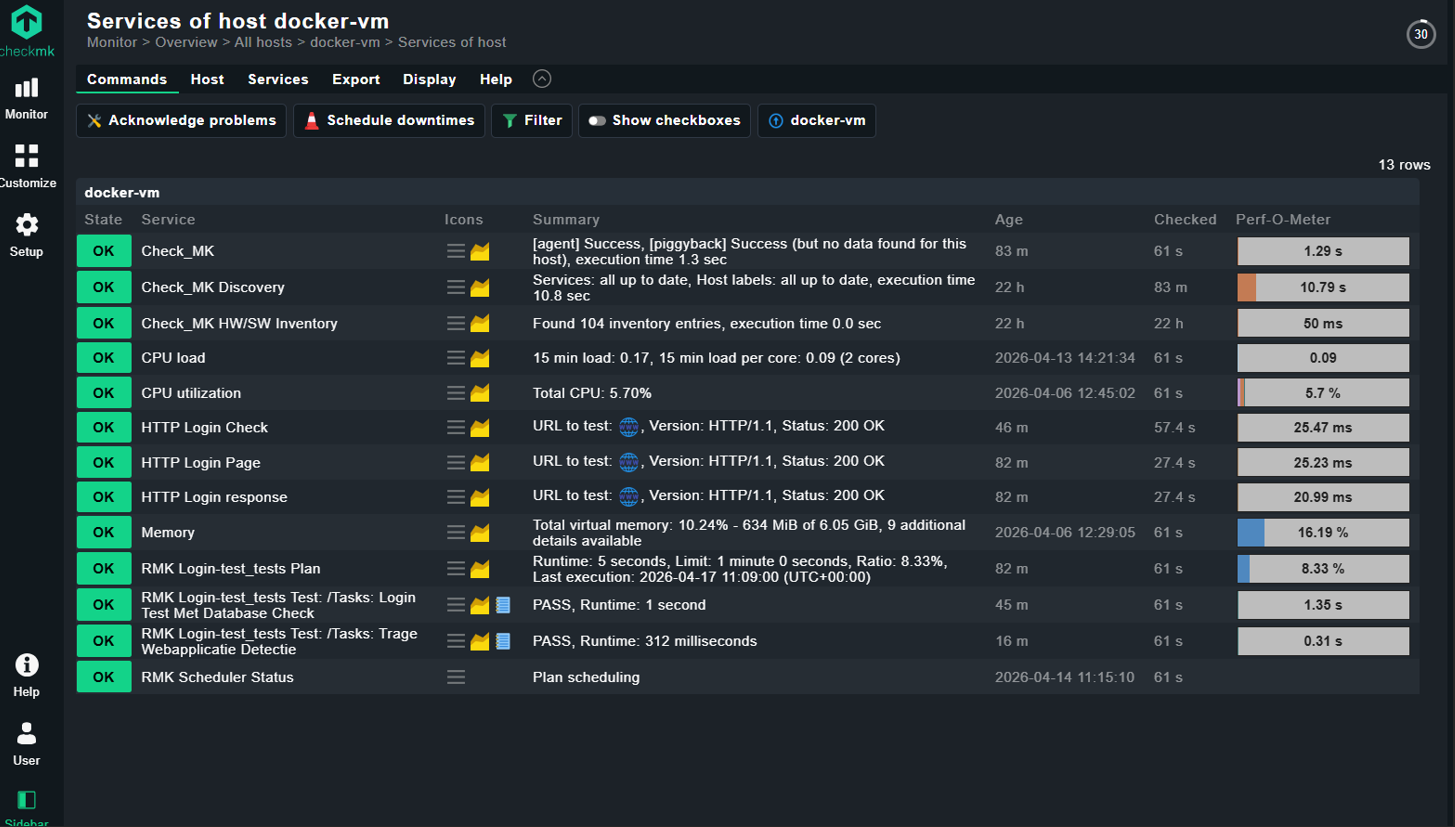
\includegraphics[width=0.85\textwidth]{e2e_scenario3_OK.png}
    \caption{Normaal verloop van de Robotmk-test zonder vertraging}
    \label{fig:e2e_scenario3_OK}
\end{figure}

\begin{figure}[H]
    \centering
    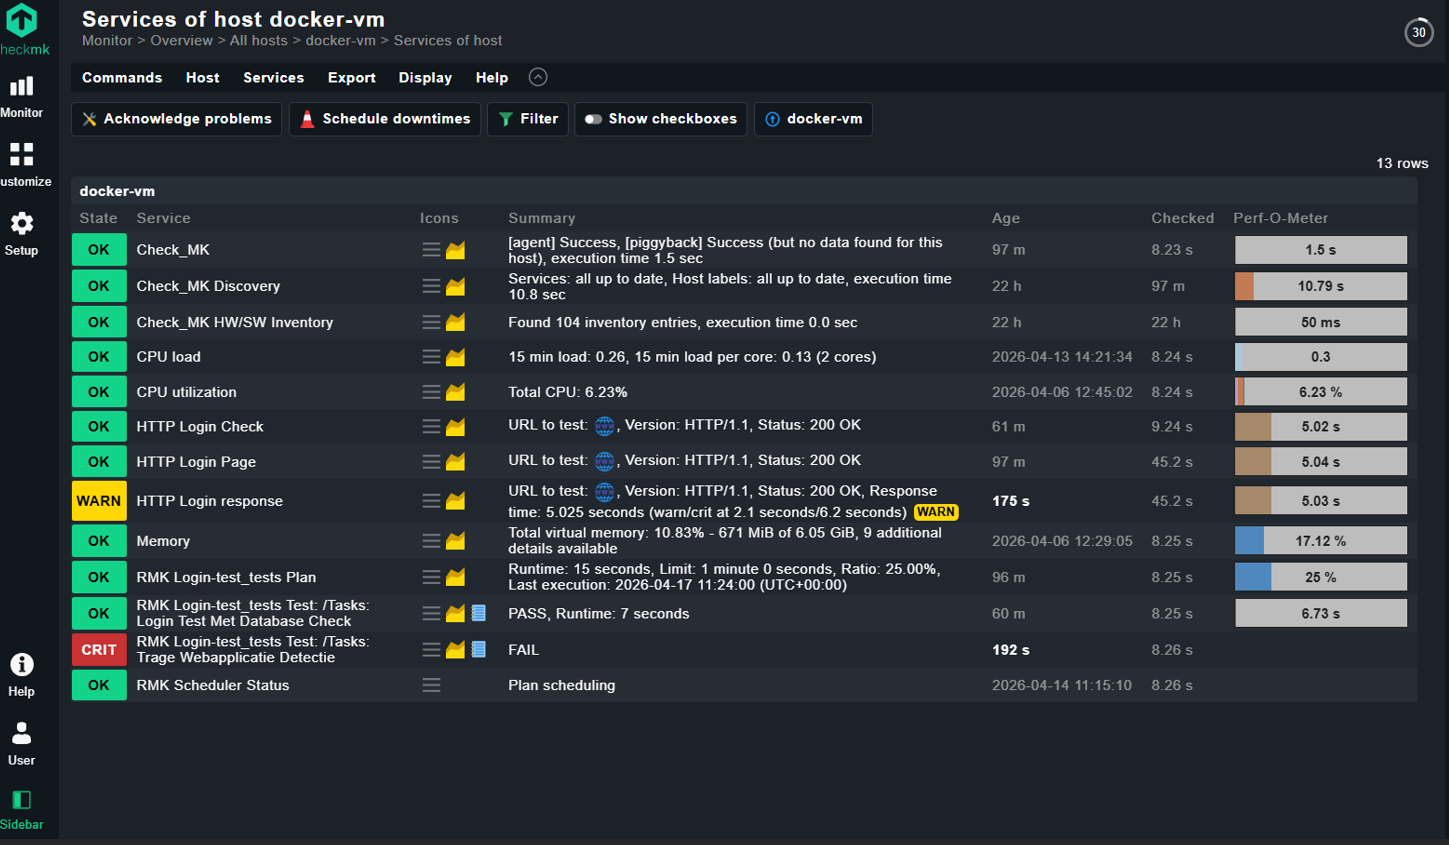
\includegraphics[width=0.85\textwidth]{e2e_scenario3_CRIT.png}
    \caption{Robotmk-test faalt doordat de laadtijd de ingestelde drempelwaarde overschrijdt}
    \label{fig:e2e_scenario3_CRIT}
\end{figure}

\begin{figure}[H]
    \centering
    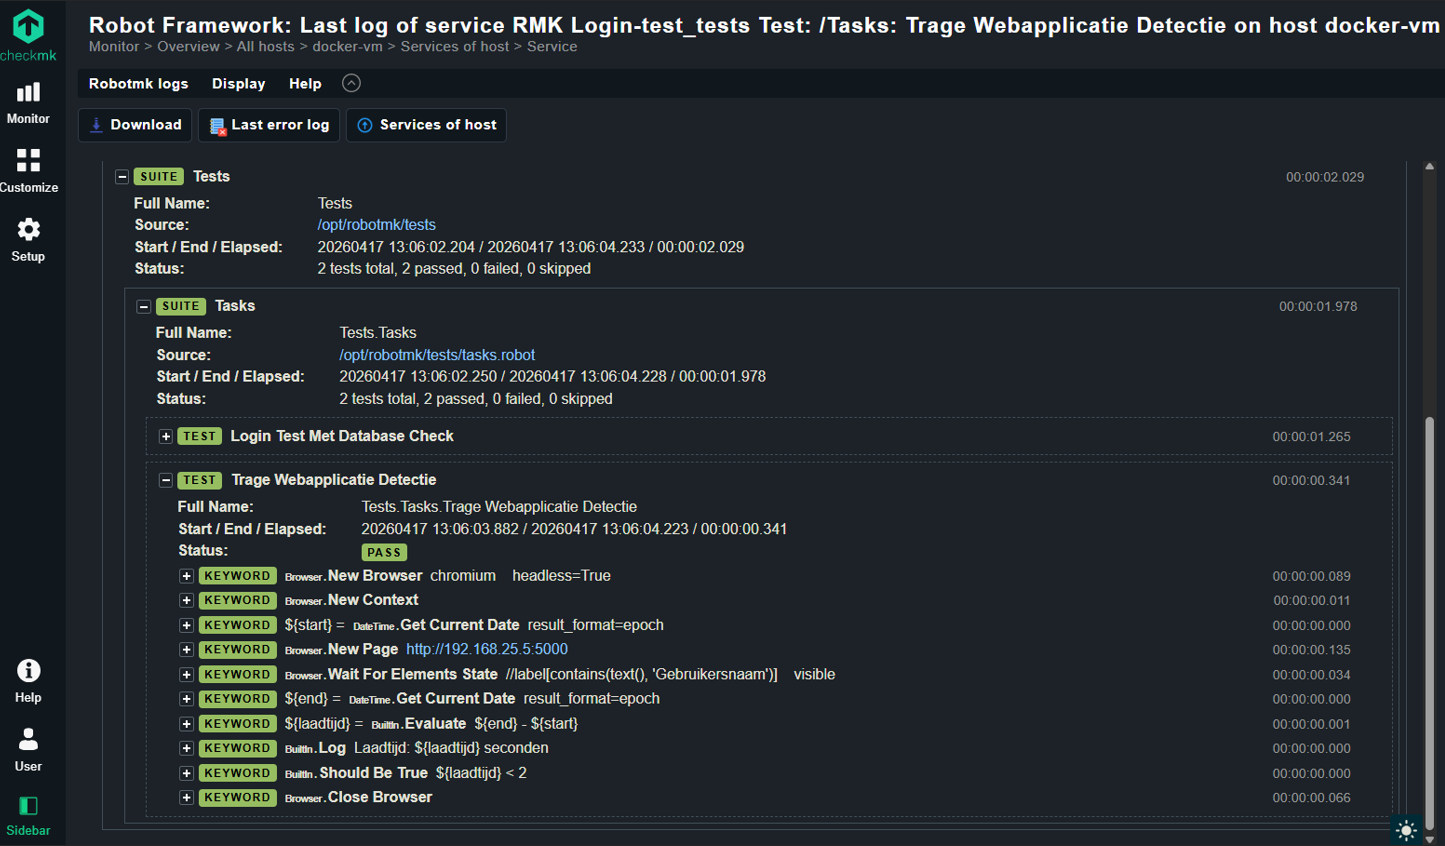
\includegraphics[width=0.85\textwidth]{e2e_scenario3_fast.png}
    \caption{Robotmk toont een normale laadtijd en detecteert geen afwijkingen}
    \label{fig:e2e_scenario3_fast}
\end{figure}

\begin{figure}[H]
    \centering
    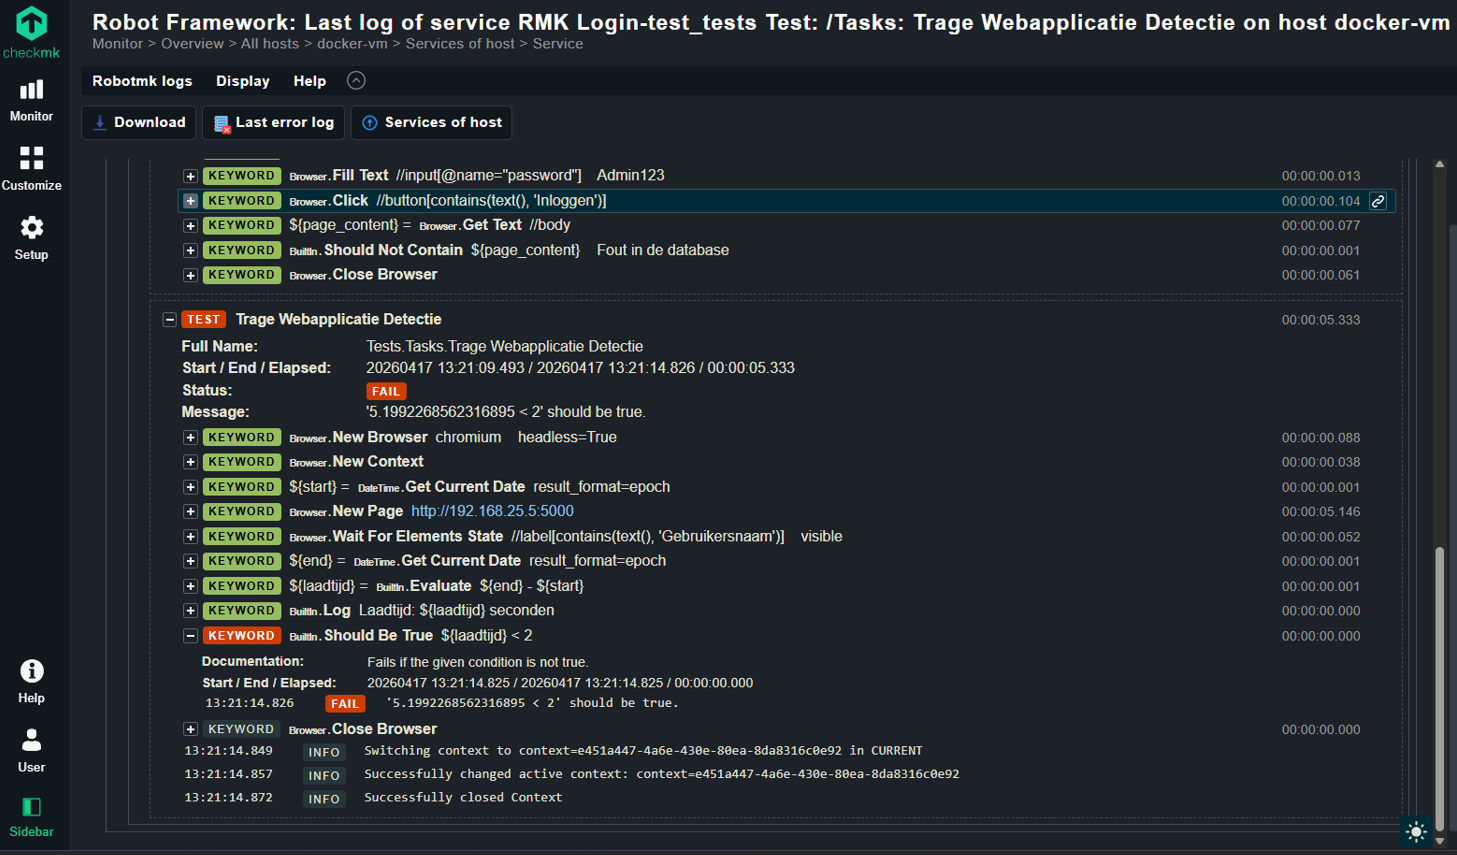
\includegraphics[width=0.85\textwidth]{e2e_scenario3_slow.png}
    \caption{Robotmk toont een verhoogde laadtijd en detecteert een trage webapplicatie}
    \label{fig:e2e_scenario3_slow}
\end{figure}

\subsubsection{Interpretatie}

Dit scenario toont aan dat end-to-end monitoring performantieproblemen detecteert op basis van de werkelijke gebruikerservaring.

In tegenstelling tot traditionele monitoring, waarbij enkel de responstijd van een service gemeten wordt, evalueert Robotmk de volledige interactie met de applicatie. Hierdoor wordt zichtbaar hoe lang een gebruiker effectief moet wachten tot de pagina bruikbaar is.

Een bijkomend voordeel is dat de testlog inzicht geeft in de duur van elke stap binnen de gebruikersflow, waardoor bepaald kan worden waar de vertraging optreedt. 

Dit maakt het mogelijk om performantieproblemen niet alleen te detecteren, maar ook gerichter te analyseren vanuit het perspectief van de eindgebruiker.

\subsection{Scenario 4: Hoge CPU-belasting (end-to-end monitoring)}

\subsubsection{Beschrijving}

In dit scenario wordt een infrastructuurprobleem gesimuleerd door de CPU-belasting van de virtuele machine te verhogen.

Het doel van dit scenario is om te onderzoeken in welke mate end-to-end monitoring in staat is om onderliggende systeemproblemen, zoals een hoge CPU-belasting, te detecteren vanuit het perspectief van de eindgebruiker.

\subsubsection{Uitvoering}

De CPU-belasting werd verhoogd door een stressprogramma uit te voeren op de virtuele machine. Hierdoor werd een groot deel van de beschikbare CPU-capaciteit gebruikt gedurende een bepaalde periode.

Tijdens deze belasting werd de Robotmk-test uitgevoerd. Deze test simuleert een gebruikersinteractie door de webapplicatie te openen en de loginflow uit te voeren.

\subsubsection{Observatie}

De Robotmk-test bleef functioneren zolang de webapplicatie correct reageerde. In de testlog is zichtbaar dat de verschillende stappen van de gebruikersflow nog steeds succesvol werden uitgevoerd.

Dit gedrag wordt geïllustreerd in Figuur~\ref{fig:e2e_scenario4_FAIL}.

\begin{figure}[H]
    \centering
    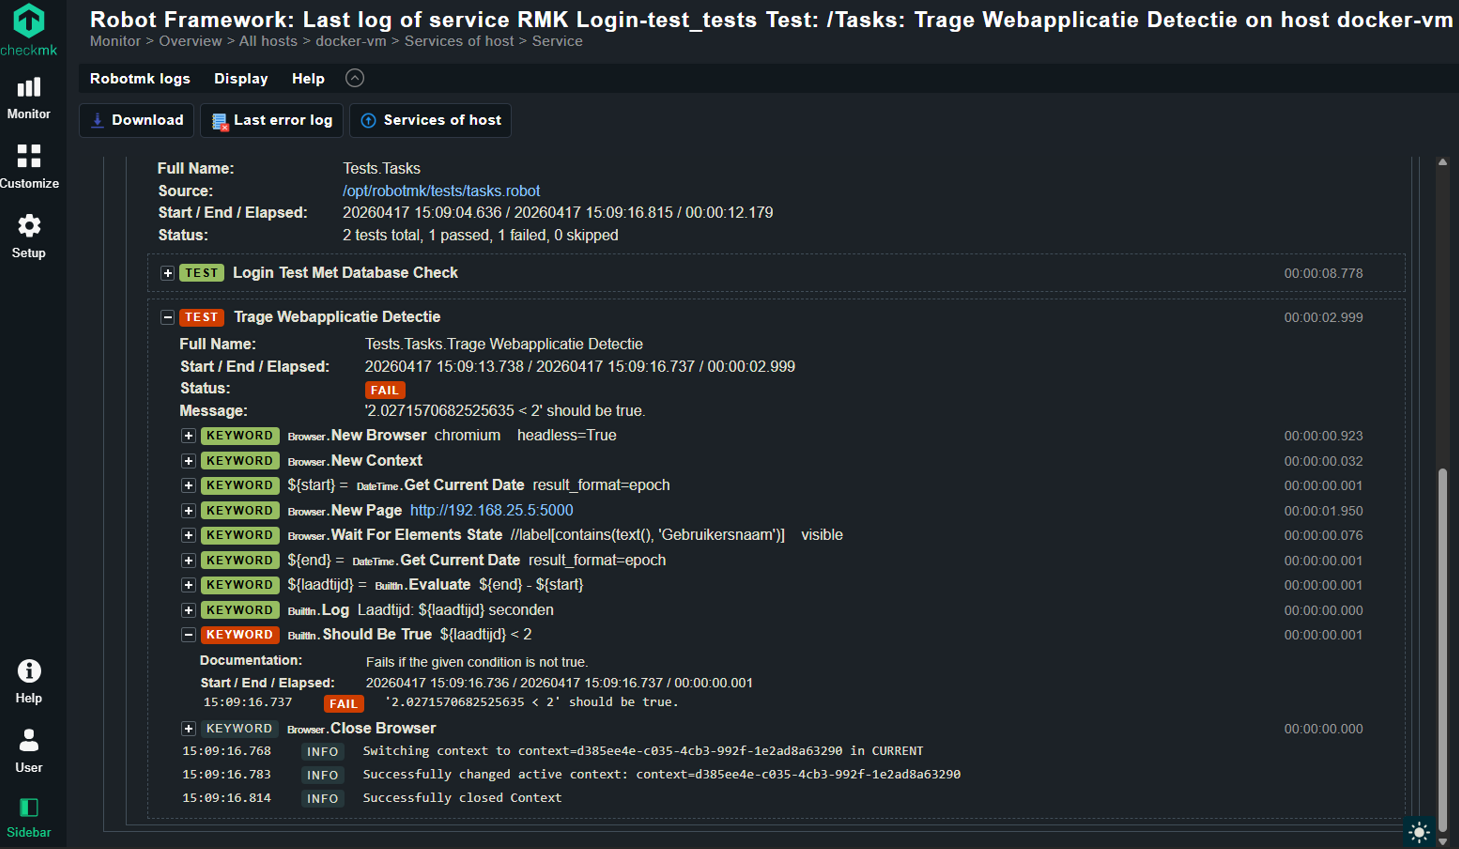
\includegraphics[width=0.85\textwidth]{e2e_scenario4_FAIL.png}
    \caption{Robotmk-test faalt doordat de responstijd de ingestelde drempelwaarde van 2 seconden overschrijdt}
    \label{fig:e2e_scenario4_FAIL}
\end{figure}

\subsubsection{Interpretatie}

Dit scenario toont aan dat end-to-end monitoring minder geschikt is voor het detecteren van infrastructuurproblemen zoals een hoge CPU-belasting.

De test toont aan dat er een vertraging is in de normale werking van de webapplicatie maar detecteert dit niet als een hoge CPU-belasting.

In tegenstelling tot traditionele monitoring, waarbij parameters zoals CPU load en CPU utilization rechtstreeks gemeten worden, richt end-to-end monitoring zich op de gebruikerservaring.

Dit toont aan dat end-to-end monitoring geen inzicht geeft in de oorzaak van het probleem, maar enkel in de impact ervan op de gebruikerservaring.

\subsection{Scenario 5: Verlies van connectiviteit tussen applicatie en database (end-to-end monitoring)}

\subsubsection{Beschrijving}

In dit scenario wordt een connectiviteitsprobleem tussen de webapplicatie en de database gesimuleerd.

Het doel van dit scenario is om te onderzoeken in welke mate end-to-end monitoring in staat is om problemen binnen de volledige gebruikersflow te detecteren wanneer de applicatie geen correcte verbinding meer kan maken met de database.

\subsubsection{Uitvoering}

De connectiviteit tussen de webapplicatie en de database werd verstoord door een foutieve configuratie van de databasehost binnen de applicatieomgeving.

Hierdoor bleef de database technisch actief, maar kon de webapplicatie geen verbinding meer maken met de database.

Tijdens dit scenario werd de Robotmk-test uitgevoerd waarbij automatisch een gebruikersinteractie met de loginflow gesimuleerd werd.

De test controleerde onder andere:
\begin{itemize}
    \item of de loginpagina correct geladen werd;
    \item of gebruikersgegevens ingevuld konden worden;
    \item of er geen foutmelding verscheen tijdens de loginprocedure.
\end{itemize}

\subsubsection{Observatie}

Tijdens de uitvoering van de loginflow stelde Robotmk vast dat de webapplicatie de foutmelding \texttt{Fout in de database} weergaf.

Hierdoor faalde de Robotmk-test en werd het probleem automatisch gedetecteerd vanuit het perspectief van de eindgebruiker.

Dit gedrag wordt geïllustreerd in Figuur~\ref{fig:e2e_scenario5_FAIL}.

\begin{figure}[H]
    \centering
    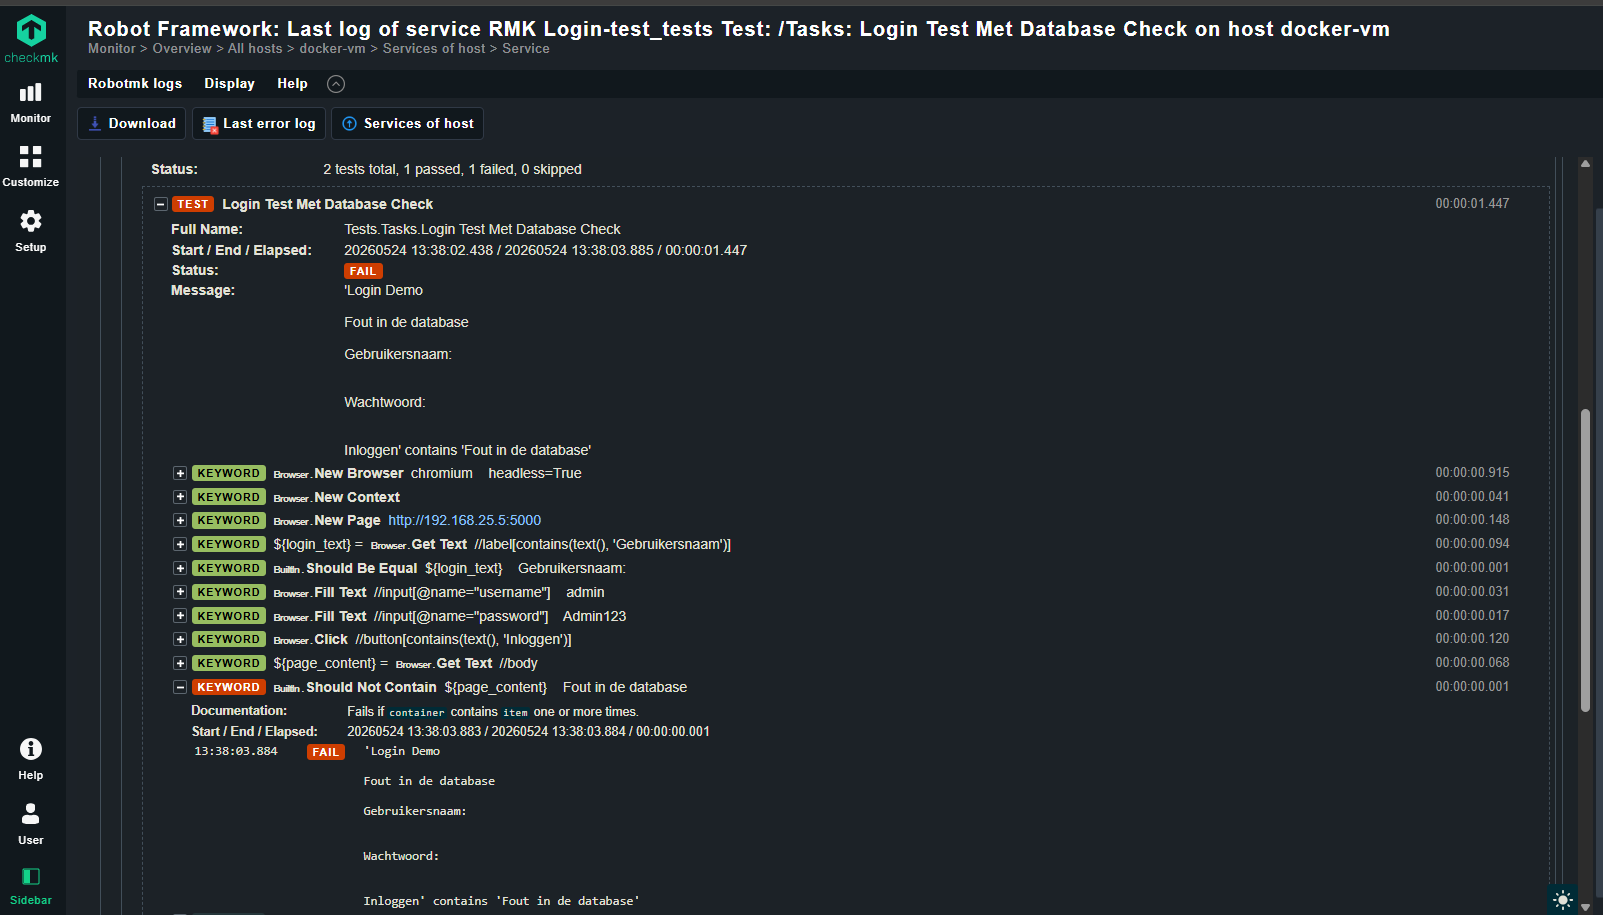
\includegraphics[width=\textwidth]{scenario5_foutflow.png}
    \caption{Overzicht van scenario 5 waarbij de database technisch actief blijft terwijl de webapplicatie geen correcte verbinding meer kan maken met de database.}
    \label{fig:e2e_scenario5_FAIL}
\end{figure}

\subsubsection{Interpretatie}

Dit scenario toont aan dat end-to-end monitoring in staat is om problemen binnen de volledige gebruikersflow automatisch te detecteren.

Hoewel de webapplicatie nog bereikbaar bleef, kon de loginflow niet correct uitgevoerd worden doordat de applicatie geen verbinding meer kon maken met de database.

Daarnaast toont dit scenario aan dat end-to-end monitoring voornamelijk inzicht biedt in de impact van een probleem op de gebruikerservaring, terwijl traditionele monitoring meer inzicht kan geven in de onderliggende technische oorzaak van het incident.

\subsection{Scenario 6: Redirectloop na login (end-to-end monitoring)}

\subsubsection{Beschrijving}

In dit scenario wordt een functioneel probleem binnen de webapplicatie gesimuleerd waarbij gebruikers na een succesvolle login opnieuw teruggestuurd worden naar de loginpagina in plaats van naar de verwachte succespagina.

Het doel van dit scenario is om te onderzoeken in welke mate end-to-end monitoring functionele problemen binnen de gebruikersflow kan detecteren vanuit het perspectief van de eindgebruiker.

\subsubsection{Uitvoering}

De applicatielogica werd aangepast zodat gebruikers na een correcte login niet doorgestuurd werden naar de succespagina, maar opnieuw op de loginpagina terechtkwamen.

Hierdoor bleef de webapplicatie technisch bereikbaar en retourneerde de webserver correcte HTTP-responses, ondanks het feit dat de loginflow functioneel niet correct werkte.

Tijdens dit scenario werd de Robotmk-test uitgevoerd waarbij automatisch een gebruikersinteractie met de loginflow gesimuleerd werd.

\subsubsection{Observatie}

Tijdens de uitvoering van de loginflow stelde Robotmk vast dat de gebruiker na het aanmelden opnieuw op de loginpagina terechtkwam in plaats van op de verwachte succespagina.

Hierdoor faalde de Robotmk-test en werd het functionele probleem automatisch gedetecteerd vanuit het perspectief van de eindgebruiker.

Dit gedrag wordt geïllustreerd in Figuur~\ref{fig:e2e_scenario6_FAIL}.

\begin{figure}[H]
    \centering
    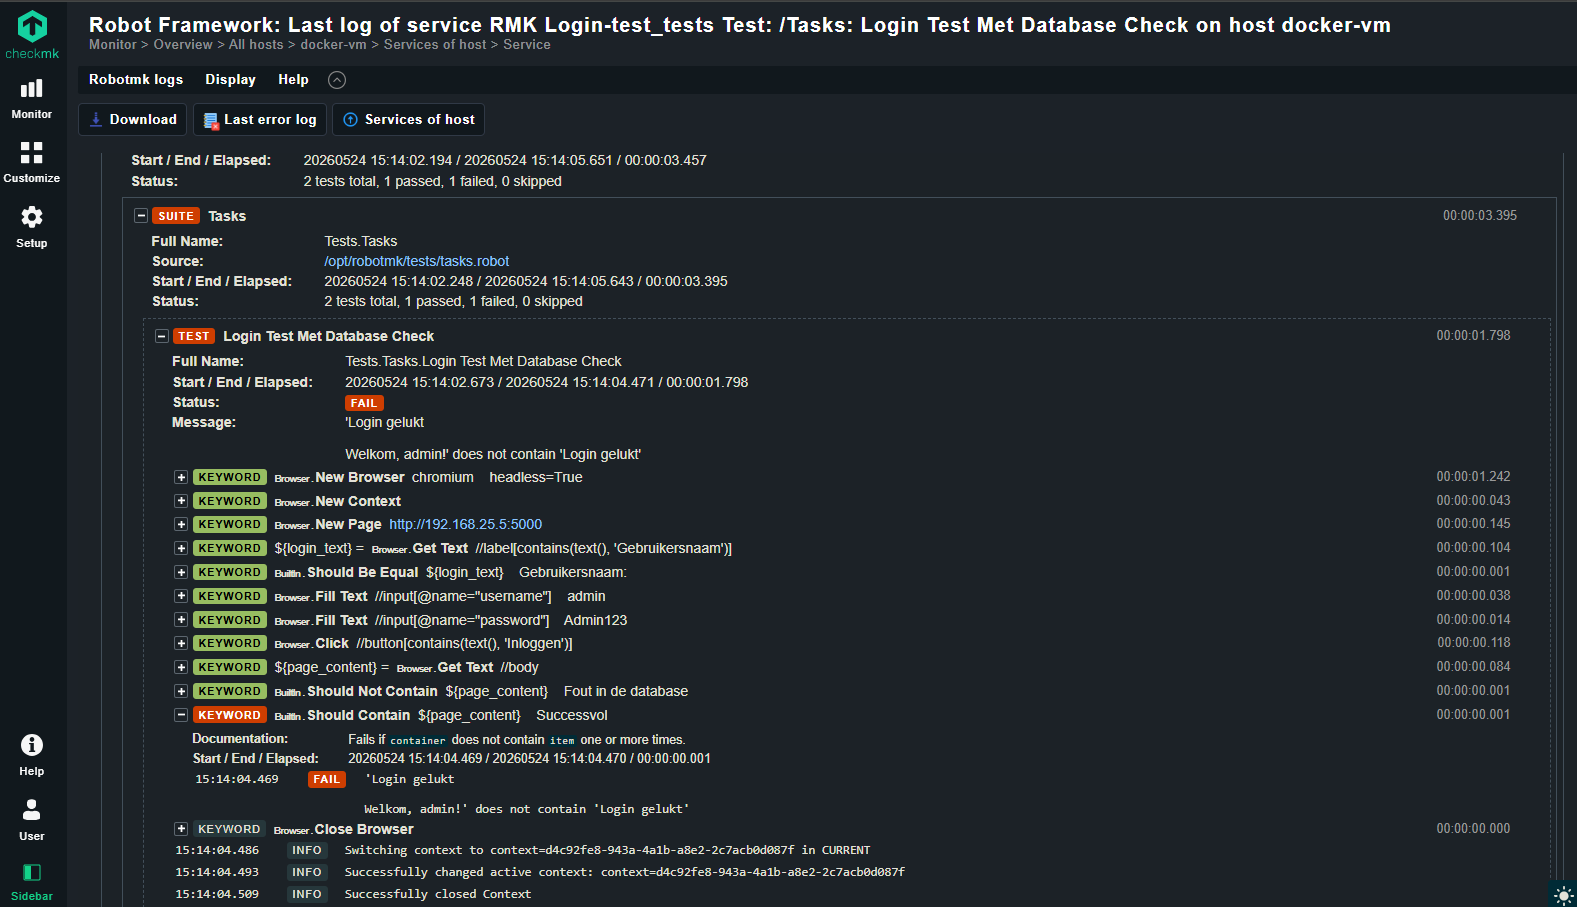
\includegraphics[width=0.9\textwidth]{Scenario6_foutflow.png}
    \caption{Robotmk-test faalt doordat de gebruiker niet op de verwachte succespagina terechtkomt}
    \label{fig:e2e_scenario6_FAIL}
\end{figure}

Na het herstellen van de applicatielogica werd de Robotmk-test opnieuw uitgevoerd. Hierbij werd de loginflow opnieuw succesvol doorlopen en kreeg de test opnieuw de status \textit{PASS}.

Dit gedrag wordt geïllustreerd in Figuur~\ref{fig:e2e_scenario6_PASS}.

\begin{figure}[H]
    \centering
    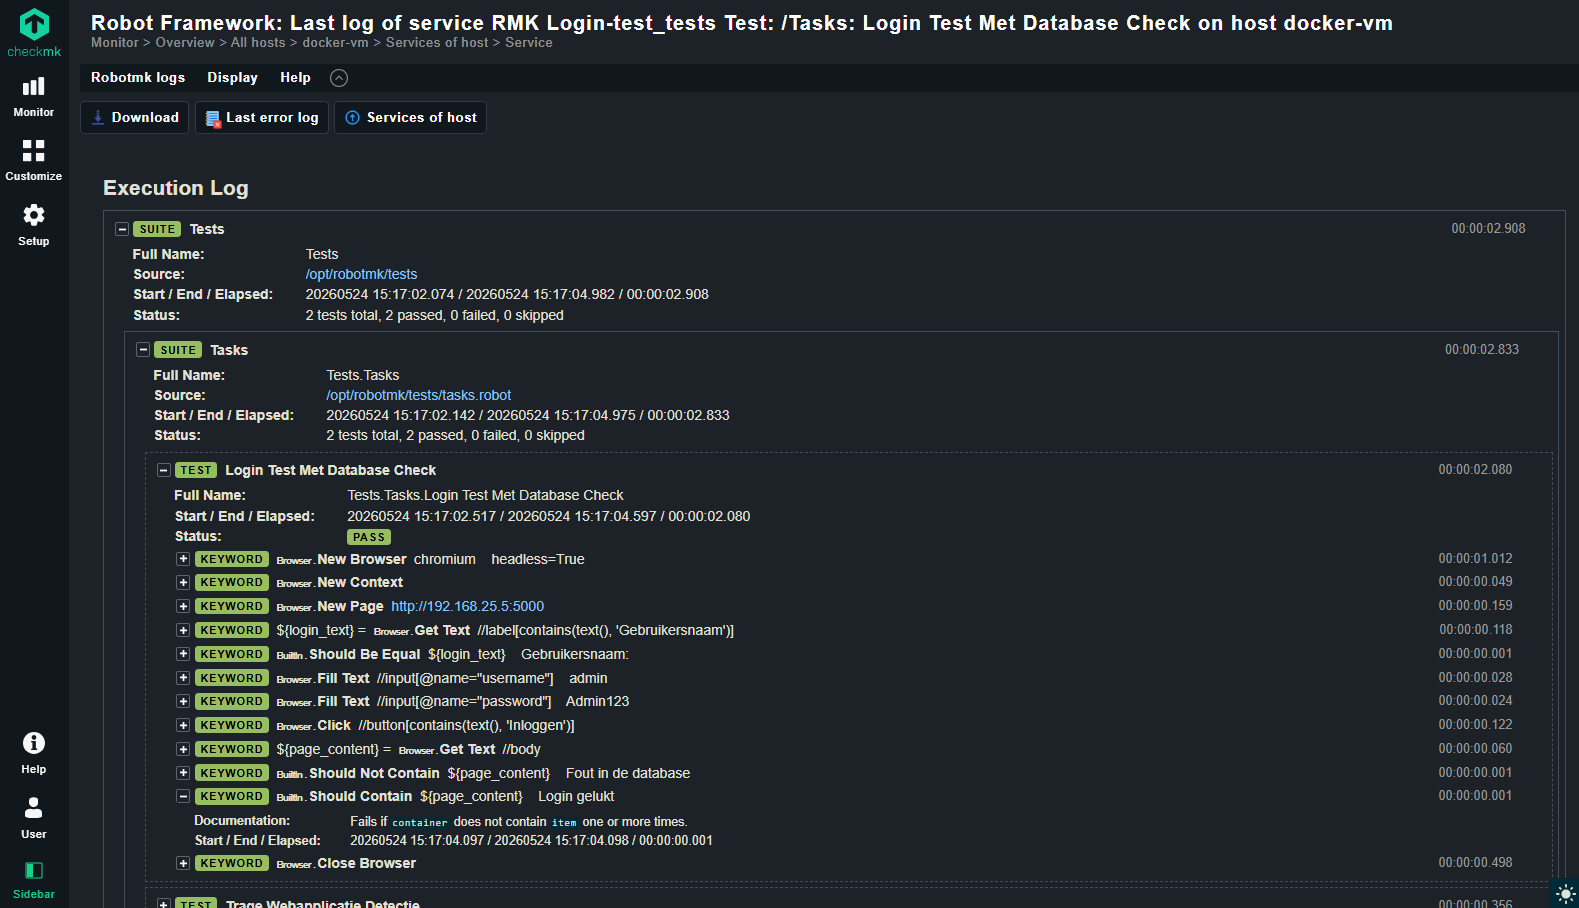
\includegraphics[width=0.9\textwidth]{Scenario6_geen_foutmelding.png}
    \caption{Robotmk-test slaagt opnieuw nadat de correcte loginflow hersteld werd}
    \label{fig:e2e_scenario6_PASS}
\end{figure}

\subsubsection{Interpretatie}

Dit scenario toont aan dat end-to-end monitoring functionele problemen binnen gebruikersflows automatisch kan detecteren vanuit het perspectief van de eindgebruiker.

Hoewel de webserver en database technisch bereikbaar bleven, werd de loginflow niet correct uitgevoerd doordat de gebruiker niet op de verwachte succespagina terechtkwam.

Dit toont aan dat end-to-end monitoring niet enkel controleert of een applicatie technisch beschikbaar blijft, maar ook of de applicatie functioneel correct werkt voor de eindgebruiker.